
\section{Experimental Results}\label{sec:experiments}
This section presents the experimental results and analyses to verify our ISC Hadoop MapReduce framework.

\subsection{Evaluation Setup}\label{subsec:evaluation_setup}

\subsubsection{System Configurations}\label{subsubsec:system_config}
For our experiments, we adopt Hadoop 0.20.205.0 as our Hadoop MapReduce framework with an input split size of 64MB by default because this has been widely adopted as a stable legacy version. 
Hadoop clusters consist of 5 nodes (1 namenode and 4 datanodes) with Intel i7 processor (3.40 GHz) and 8 GB memory running Ubuntu 12.04 LTS (64 bits). Each node is equipped with an ISC device of a 400GB SLC SSD with SAS 6Gb interface. This ISC device is connected to each node via a SAS Host Bus Adapter (HBA) with 6Gb, i.e., the host I/O bandwidth is 750 MB/s theoretically. The internal bandwidth of this SSD offers 3.2 GB/s, thus the bandwidth ratio is 4.27$\times$ theoretically\footnote{\small Our measured bandwidth ratio is around 3.8$\times$, which is a little smaller than 4.27$\times$ due to the extra firmware overhead inside SSDs.}. Since ISC features inside ISC devices are enabled/disabled from the host, this ISC device is identical to a regular SSD.

For a single node setup, we install two ISC devices to the node and run 3 node instances (1 namenode and 2 datanodes) in a single machine based on our study (please refer to subsection~\ref{subsubsec:singlenode}). This simulates Hadoop clusters of 3 nodes for a fully distributed mode. We assign one Mapper to each ISC device and configure Hadoop with two Reducers in this single node (i.e., two Mappers and two Reducers) for our initial study. All other configurations are exactly the same as the cluster setup for fair evaluation. We employ various synthetic data which are based on PUMA benchmark and vary in size from 1GB to 16GB. We can adopt another data of a bigger size, but we found those are enough to get meaningful implication and projection to such bigger data.  
We run all our experiments 30 times for statistical significance and produce a value of an average.


As our baseline system, we adopt a typical Hadoop MapReduce system with SSDs running all Mappers and Reducers in the host side. That is, for fairness, we employee the exactly same system as the ISC Hadoop MapReduce system described above except only for disabling ISC features inside our SSDs. Consequently, this ISC SSDs work as typical SSDs and the host Hadoop system run all Mappers and Reducers in the host side like a typical Hadoop system.


\subsubsection{Performance Metrics}\label{subsubsec:performance_metrics}
We mainly measure an elapsed time (seconds) as our Hadoop system performance metrics and collect all execution time information from Hadoop JobHistoryServer thereby using \emph{'hadoop job -history'} command. 


First of all, we measure an end-to-end elapsed time. This corresponds to a total execution time of a Hadoop application and includes all setup, map, shuffle, reduce, and cleanup time. This performance represents an actual application performance where end users can be conscious of the system performance gain. To deeply analyze, we delve into Mapper because our ISC Hadoop framework offload Mapper to the ISC device and the performance gain is primarily originated from the Mapper inside our ISC devices. 

An energy consumption is also another important factor. We measure the energy consumption (joule) with a Yokogawa WT330 power meter~\cite{Powermeter:Yokogawa:techspec} as follows. Once all systems are sufficiently stabilized (i.e., idle), we measure the power in Watts ($W_1$). Then while running the systems, we measure the power (assuming $W_2$) during its execution time ($t$). Now energy consumption in Joules can be drawn by $(W_2-W_1)\times t$.



\subsection{Evaluation Results}\label{subsec:evaluation_results}

\subsubsection{ISC Hadoop Demonstration}\label{subsubsec:ISC_demo}
We first start to exhibit a Hadoop system demonstration to compare our ISC Hadoop system with a typical Hadoop system. Figure~\ref{fig:ISC_Hadoop_demo} captures this demonstration. We set up both Hadoop systems on a single node with a configuration of two datanodes and one namenode as described in section~\ref{subsubsec:system_config}, and run Hadoop wordcount application with same data at the same time. Both systems are connected to a SAS/SATA bus analyzer to observe an amount of data transfer from devices to a host system. As shown in the Figure, our ISC Hadoop system completes the task two times faster than a typical Hadoop system. Moreover, we clearly observe the ISC system very rarely transfers data from the device to the host.
Now we make a variety of analyses of this result via extensive experiments.


\begin{figure}[htbp]
	\centering
		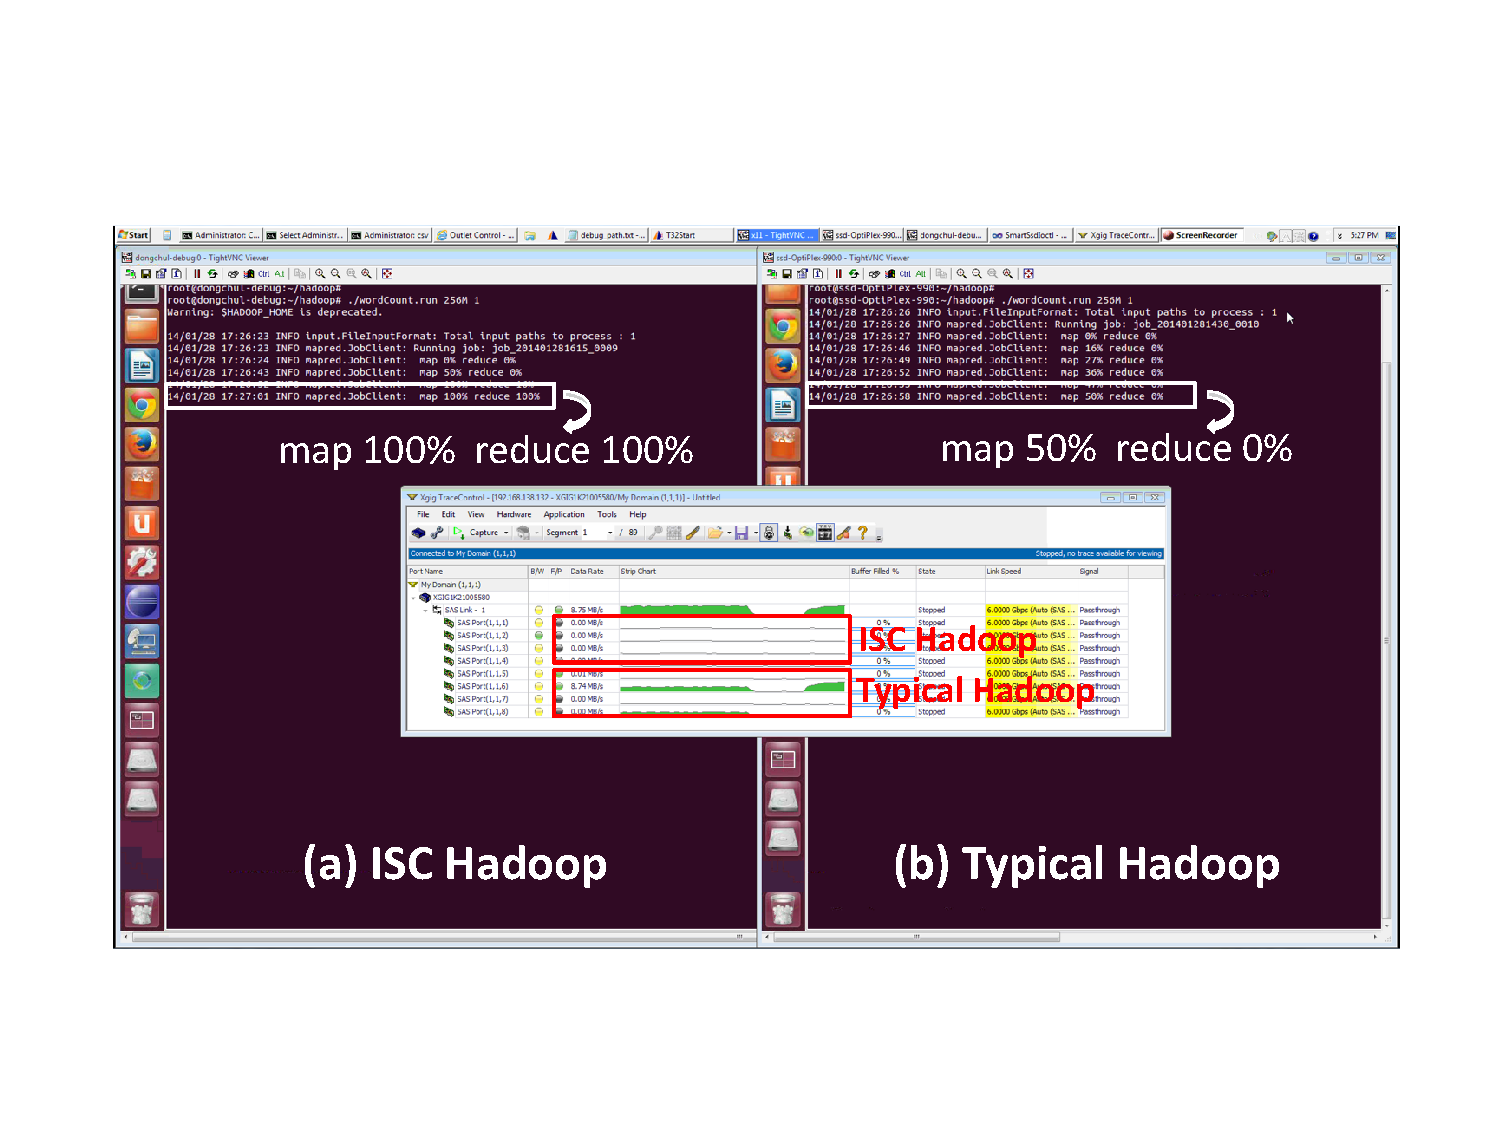
\includegraphics[width=1.0\columnwidth]{figures/ISC_Hadoop_demo.pdf}
	\caption{Hadoop System Demonstration (ISC Hadoop vs. Typical Hadoop)}
	\label{fig:ISC_Hadoop_demo}
\end{figure}







\begin{figure*}[t]
  \centering
  \renewcommand{\tabcolsep}{0.1mm}
  \begin{tabular}{ccc}
 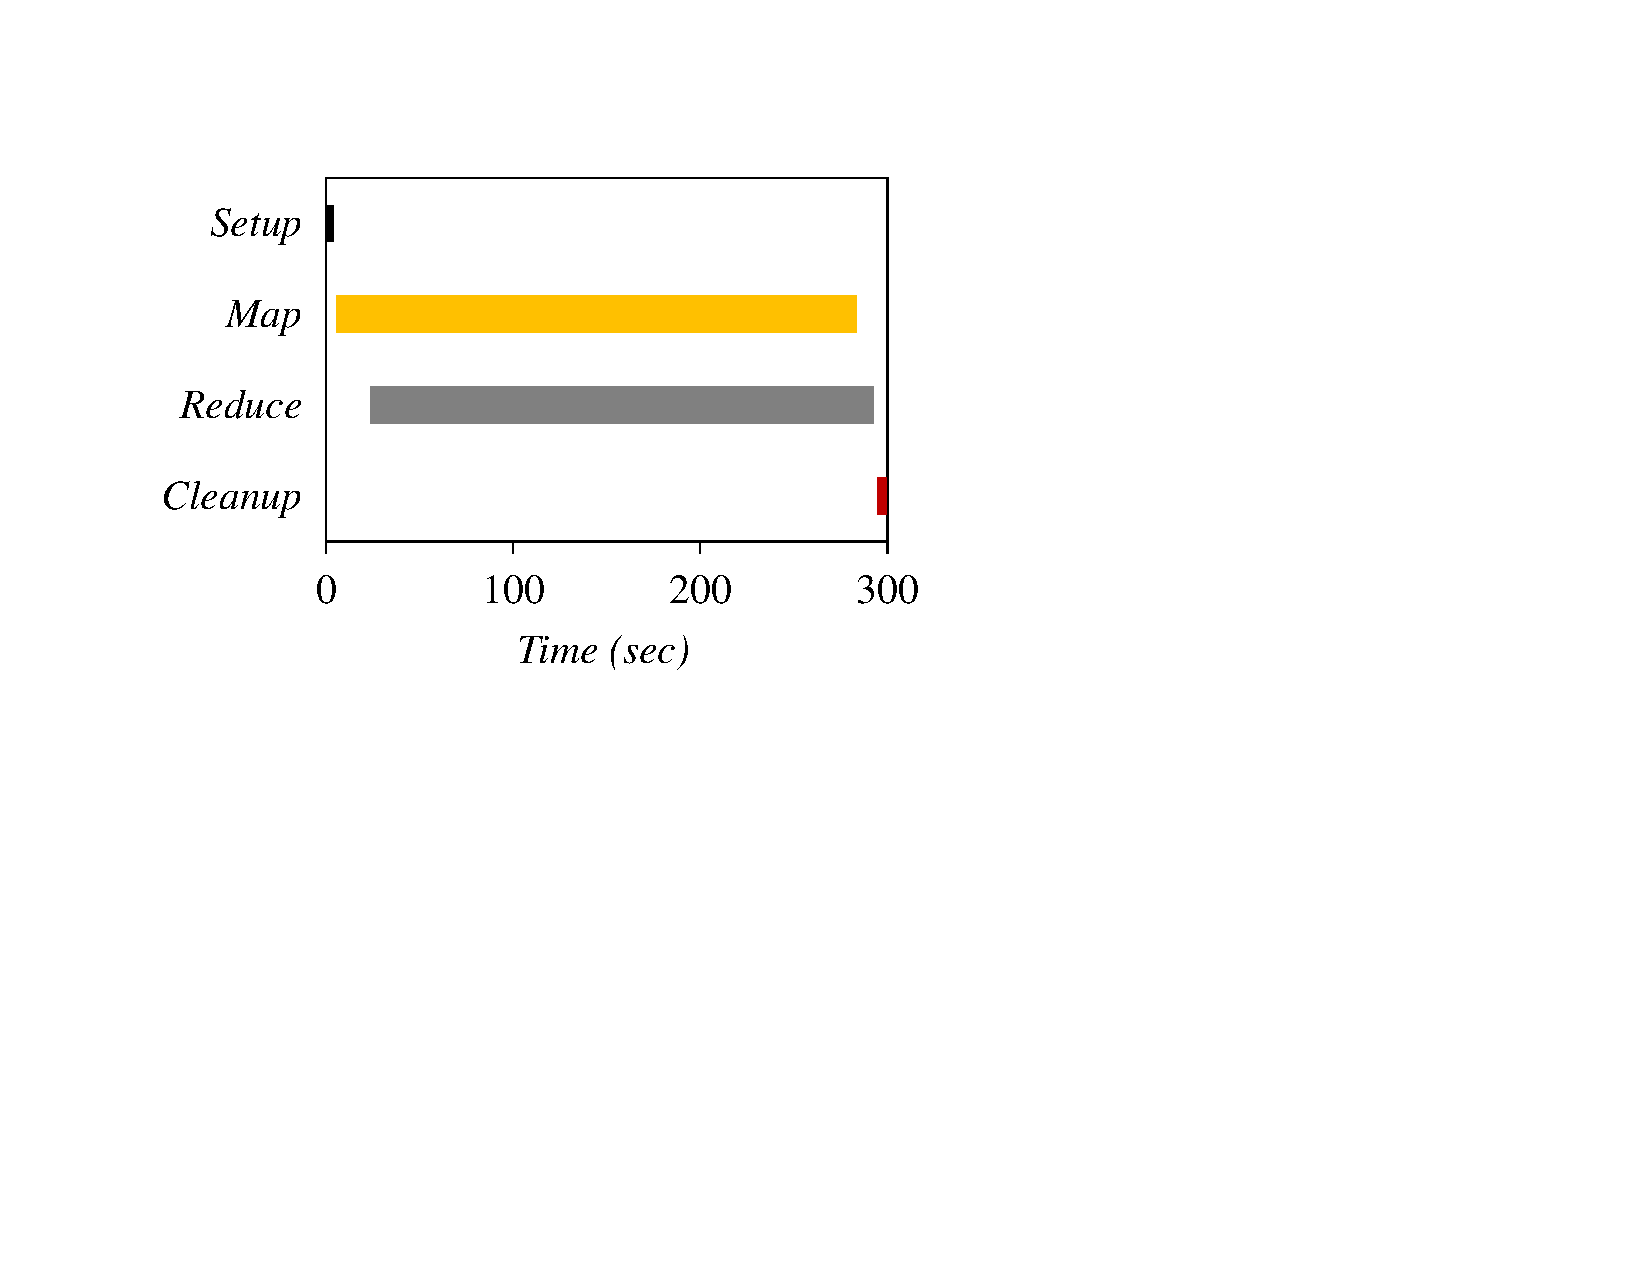
\includegraphics[width=0.69\columnwidth]{figures/Hadoop_execution_time_each_phase_breakdown2.pdf}&
  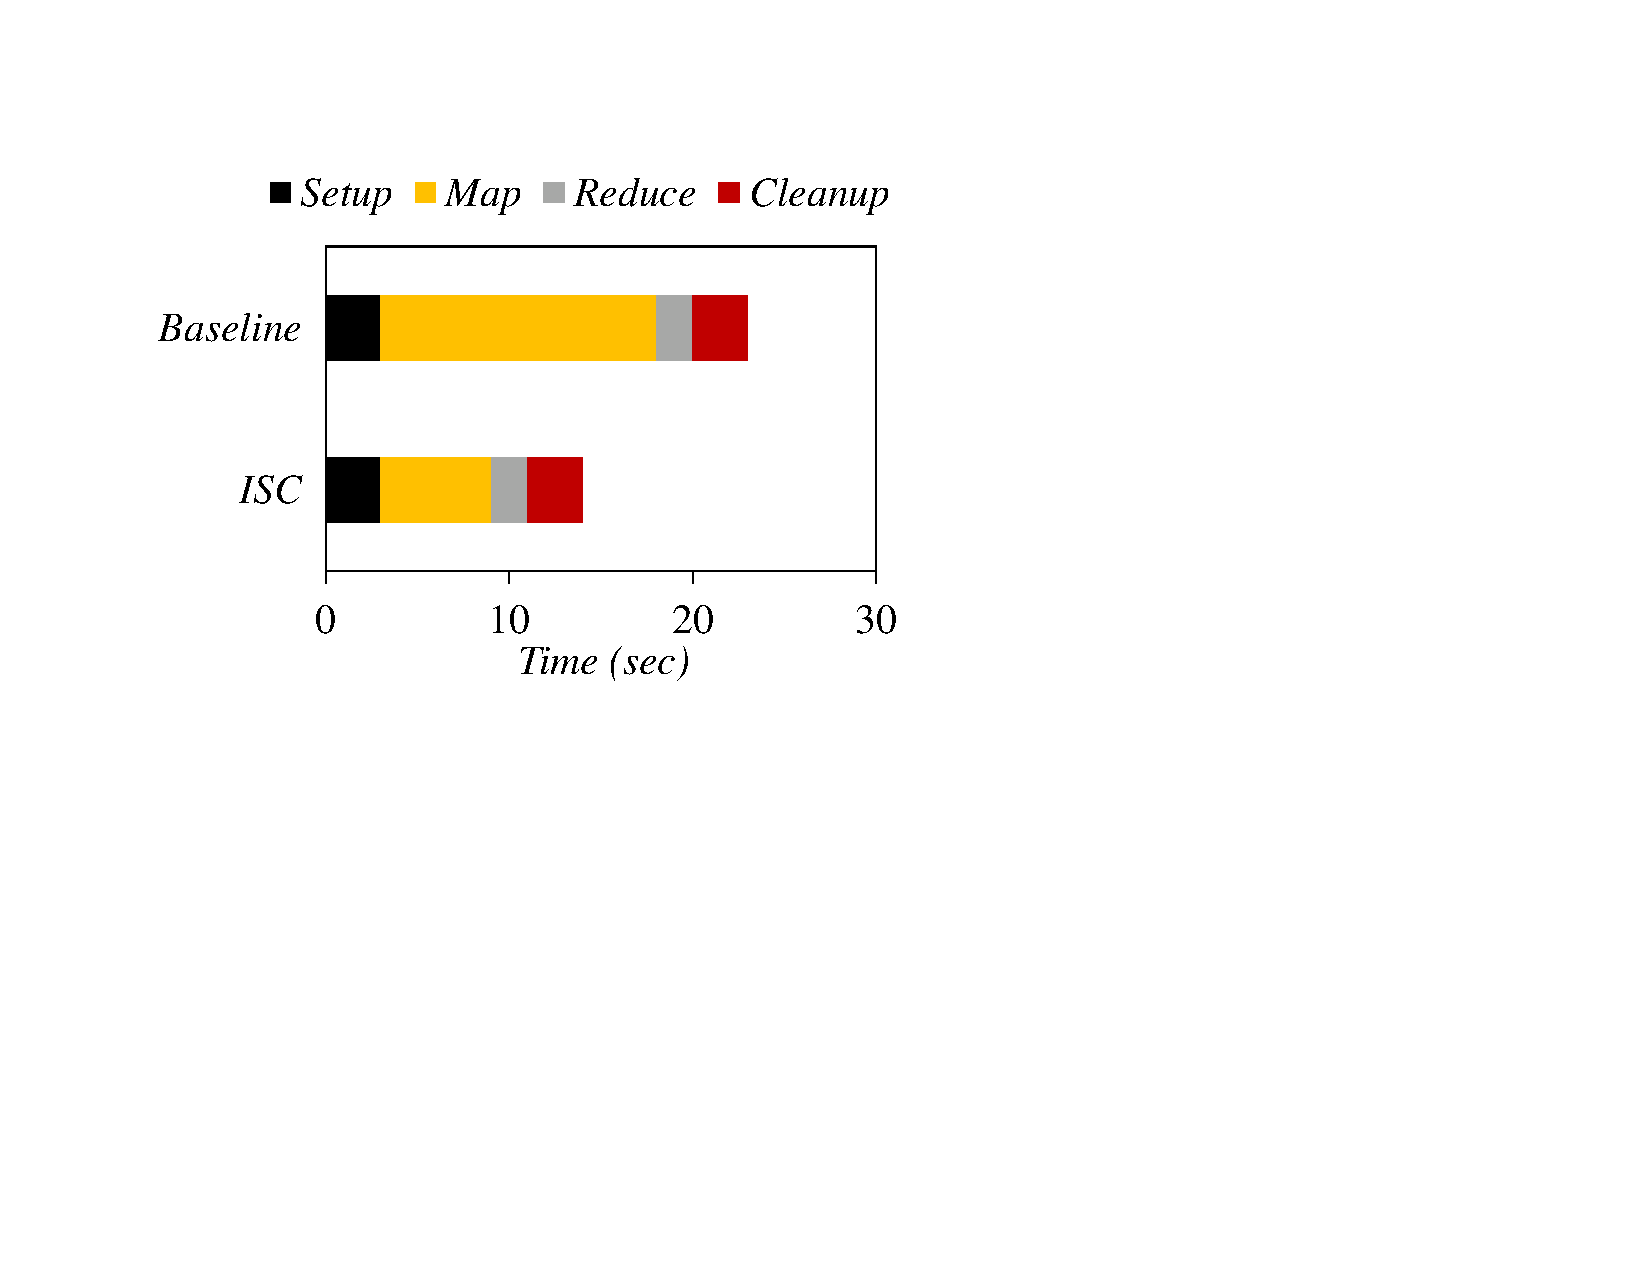
\includegraphics[width=0.69\columnwidth]{figures/Hadoop_time_breakdown1.pdf}&
  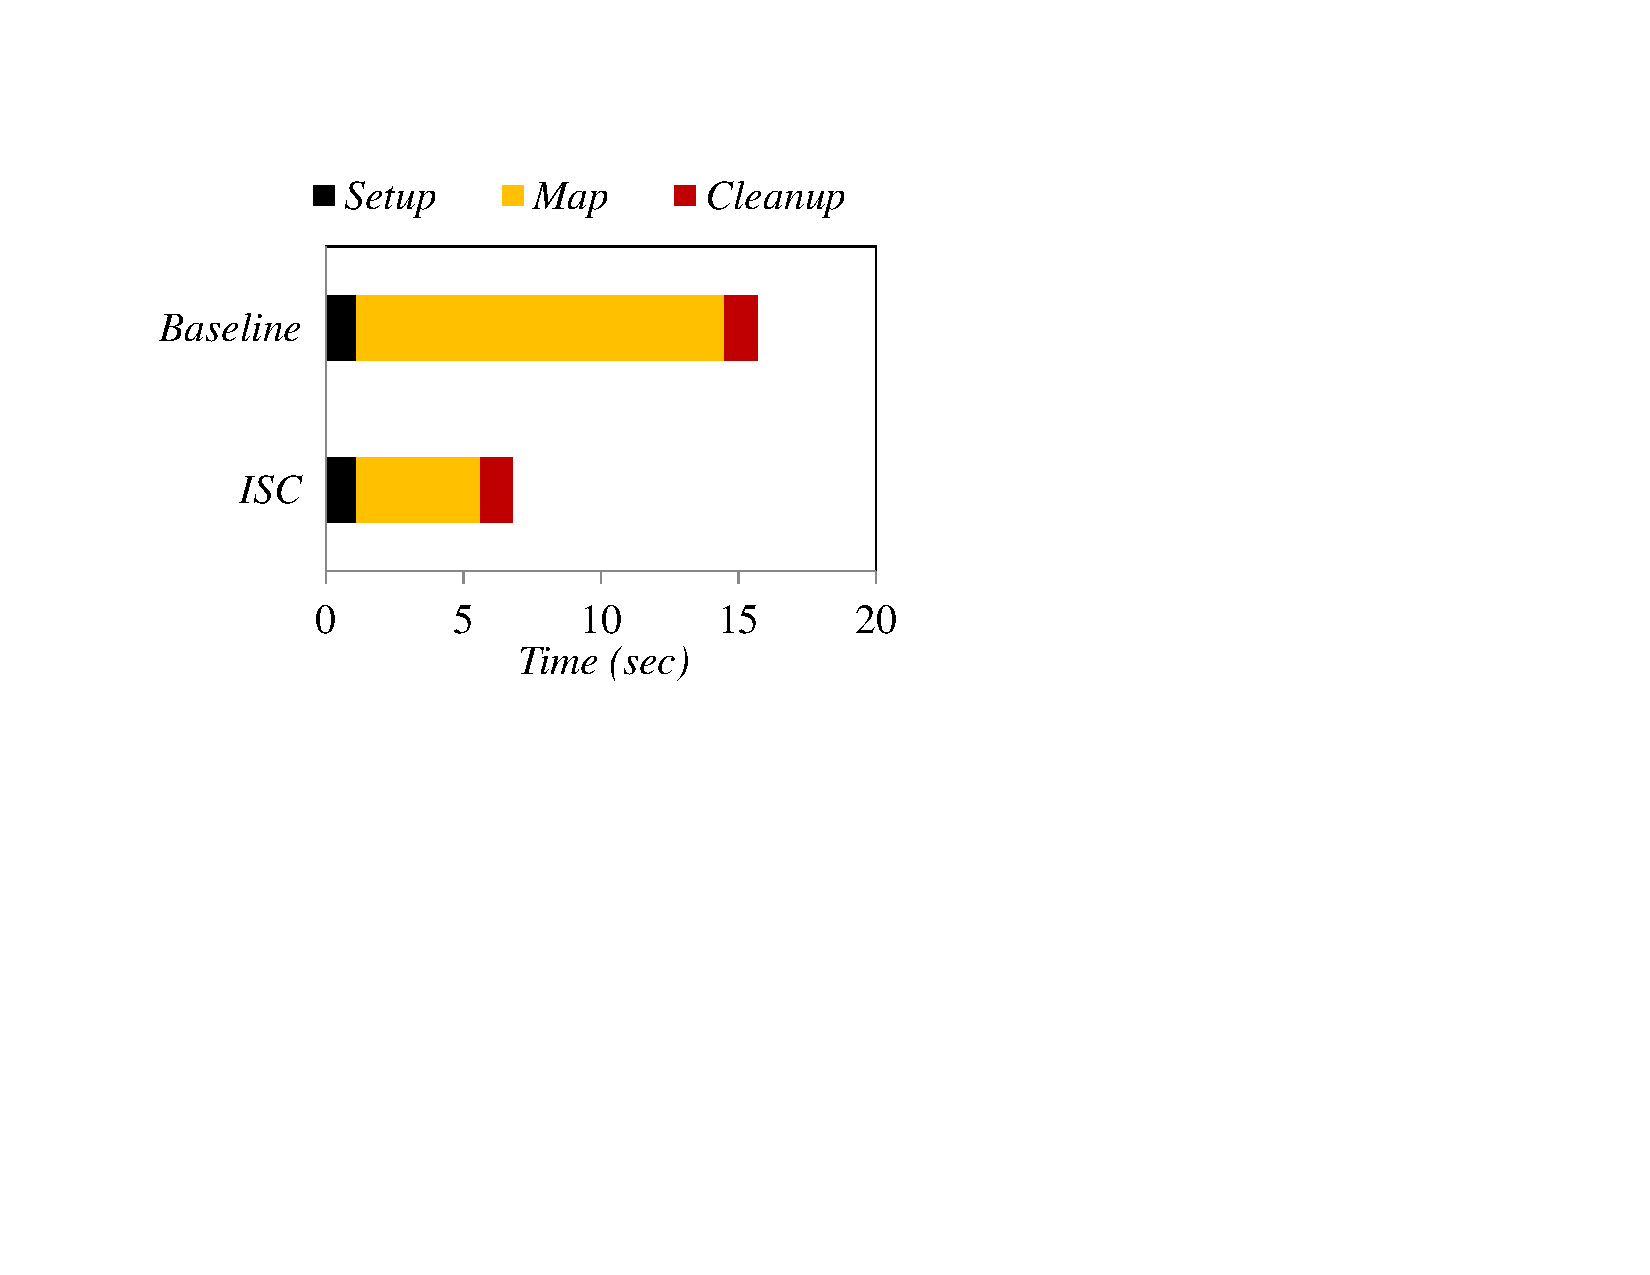
\includegraphics[width=0.69\columnwidth]{figures/Hadoop_breakdown_per_maptask1.pdf}\\	
  (a) Per Job & (b) Per Task & (c) Per Map Task
\end{tabular}
  \caption{Breakdown of each Hadoop execution time}
  \label{fig:time_breakdown}
 \end{figure*}




\subsubsection{A Single Node}\label{subsubsec:Exp_result_singlenode}
We set up two Hadoop systems for the fully distributed mode on a single node: (1) a single instance of both namenode and datanode (this corresponds to a pseudo distributed mode) and (2) a single instance of namenode and two instances of datanode. 








\begin{figure}[t]
  \centering
  \renewcommand{\tabcolsep}{0.1mm}
  \begin{tabular}{ccc}
 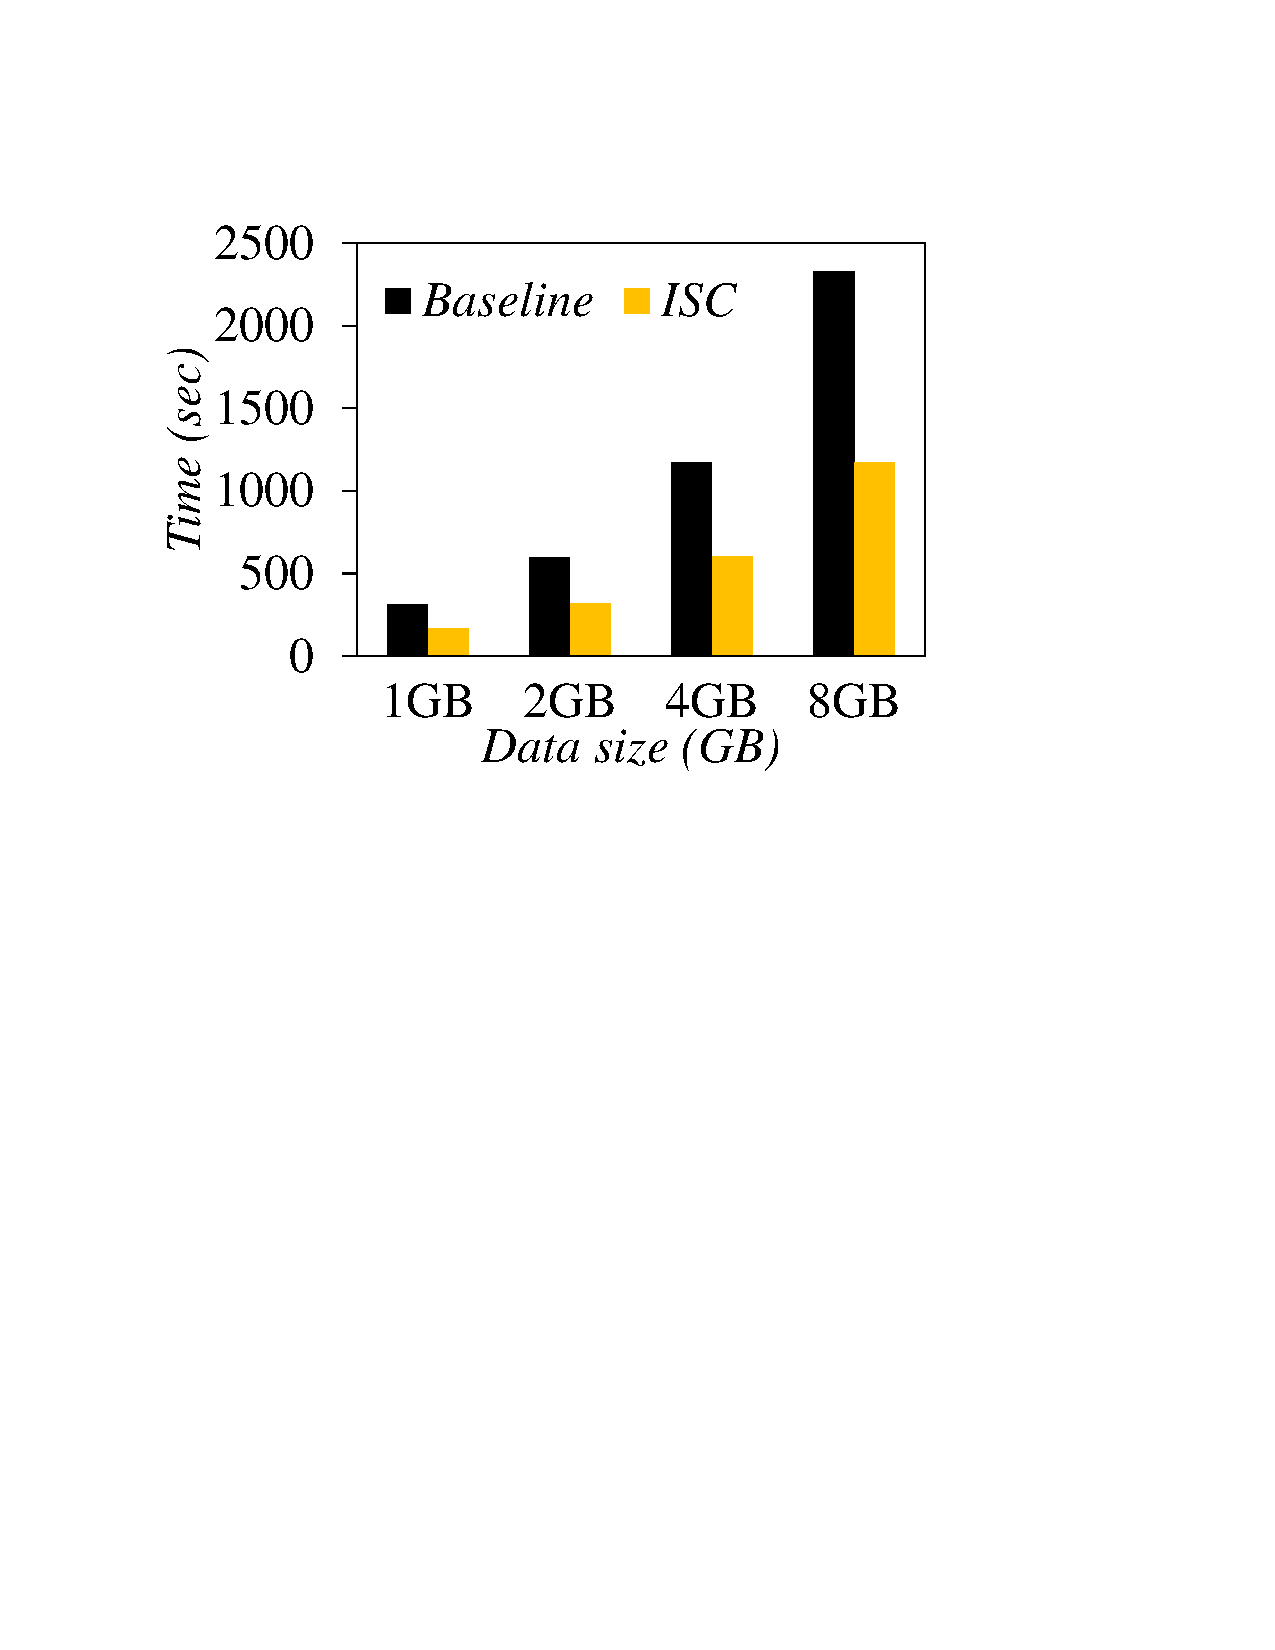
\includegraphics[width=0.5\columnwidth]{figures/Singlenode_Total_Elapsed_Time.pdf}&
  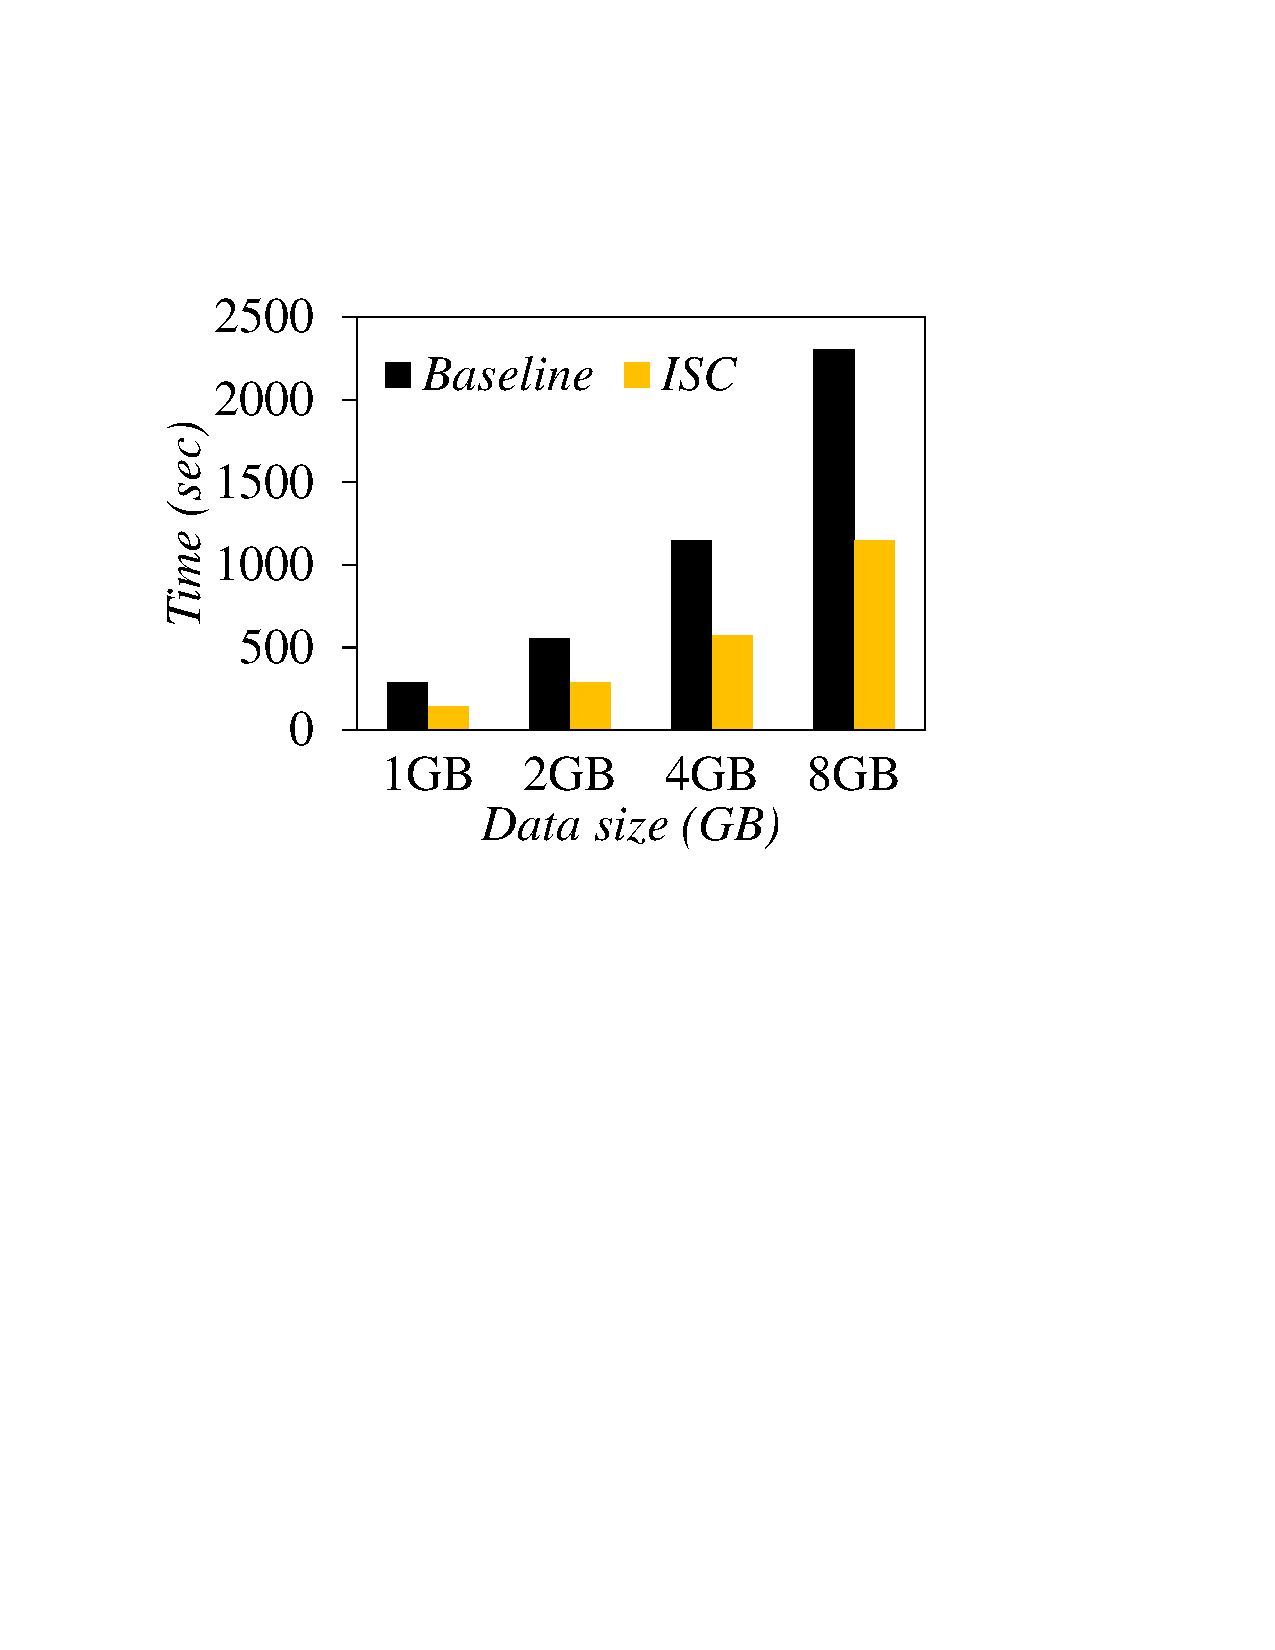
\includegraphics[width=0.5\columnwidth]{figures/Singlenode_Total_Mapper_Elapsed_Time.pdf}\\
  (a) Total Elapsed Time & (b) Total Mapper Elapsed Time
\end{tabular}
  \caption{Total elapsed time on a single node (single datanode and single namenode)}
  \label{fig:execution_time_with_single_namenode_on_single_node}
 \end{figure}






\textbf{Total elapsed time:} Figure~\ref{fig:execution_time_with_single_namenode_on_single_node} shows a total elapsed time on a single node with a single namenode and datanode. Our ISC Hadoop system achieves 2$\times$ faster than the typical Hadoop system in terms of a total elapsed time (i.e. end-to-end total execution time) (please refer to Figure~\ref{fig:execution_time_with_single_namenode_on_single_node} (a)). Figure~\ref{fig:execution_time_with_single_namenode_on_single_node} (b) displays a total elapsed time in a Mapper phase by excluding all other phases. This shows how much time each Hadoop system consumes to complete all Map tasks. Similarly, our ISC Hadoop system completes all Map tasks 2$\times$ faster than the baseline system. The results and trends in Figure~\ref{fig:execution_time_with_single_namenode_on_single_node} (b) are almost identical to those in Figure~\ref{fig:execution_time_with_single_namenode_on_single_node} (a). This is because the total execution time of all Map tasks is a significantly dominant factor of the total Hadoop running time in wordcount-like Hadoop applications (for instance, 91\% with 1GB data -- 98\% with 8GB data of the total wordcount execution time).
Figure~\ref{fig:time_breakdown} (a) demonstrates well this analysis. It breaks down the total execution time of wordcount into each Hadoop phase (baseline with 1GB data on a single node). After a short Hadoop setup time (3 seconds), the Hadoop system keeps executing each Map task (277 seconds) and completed Map tasks trigger executing a corresponding Reduce task with their output data in parallel. The total execution time of Reduce tasks (268 seconds) almost overlaps with that of Map task since it is heavily dependent on Map task completion. Lastly, Hadoop cleanup time takes about 3 seconds. 




%\begin{figure}[htbp]
%	\centering
%		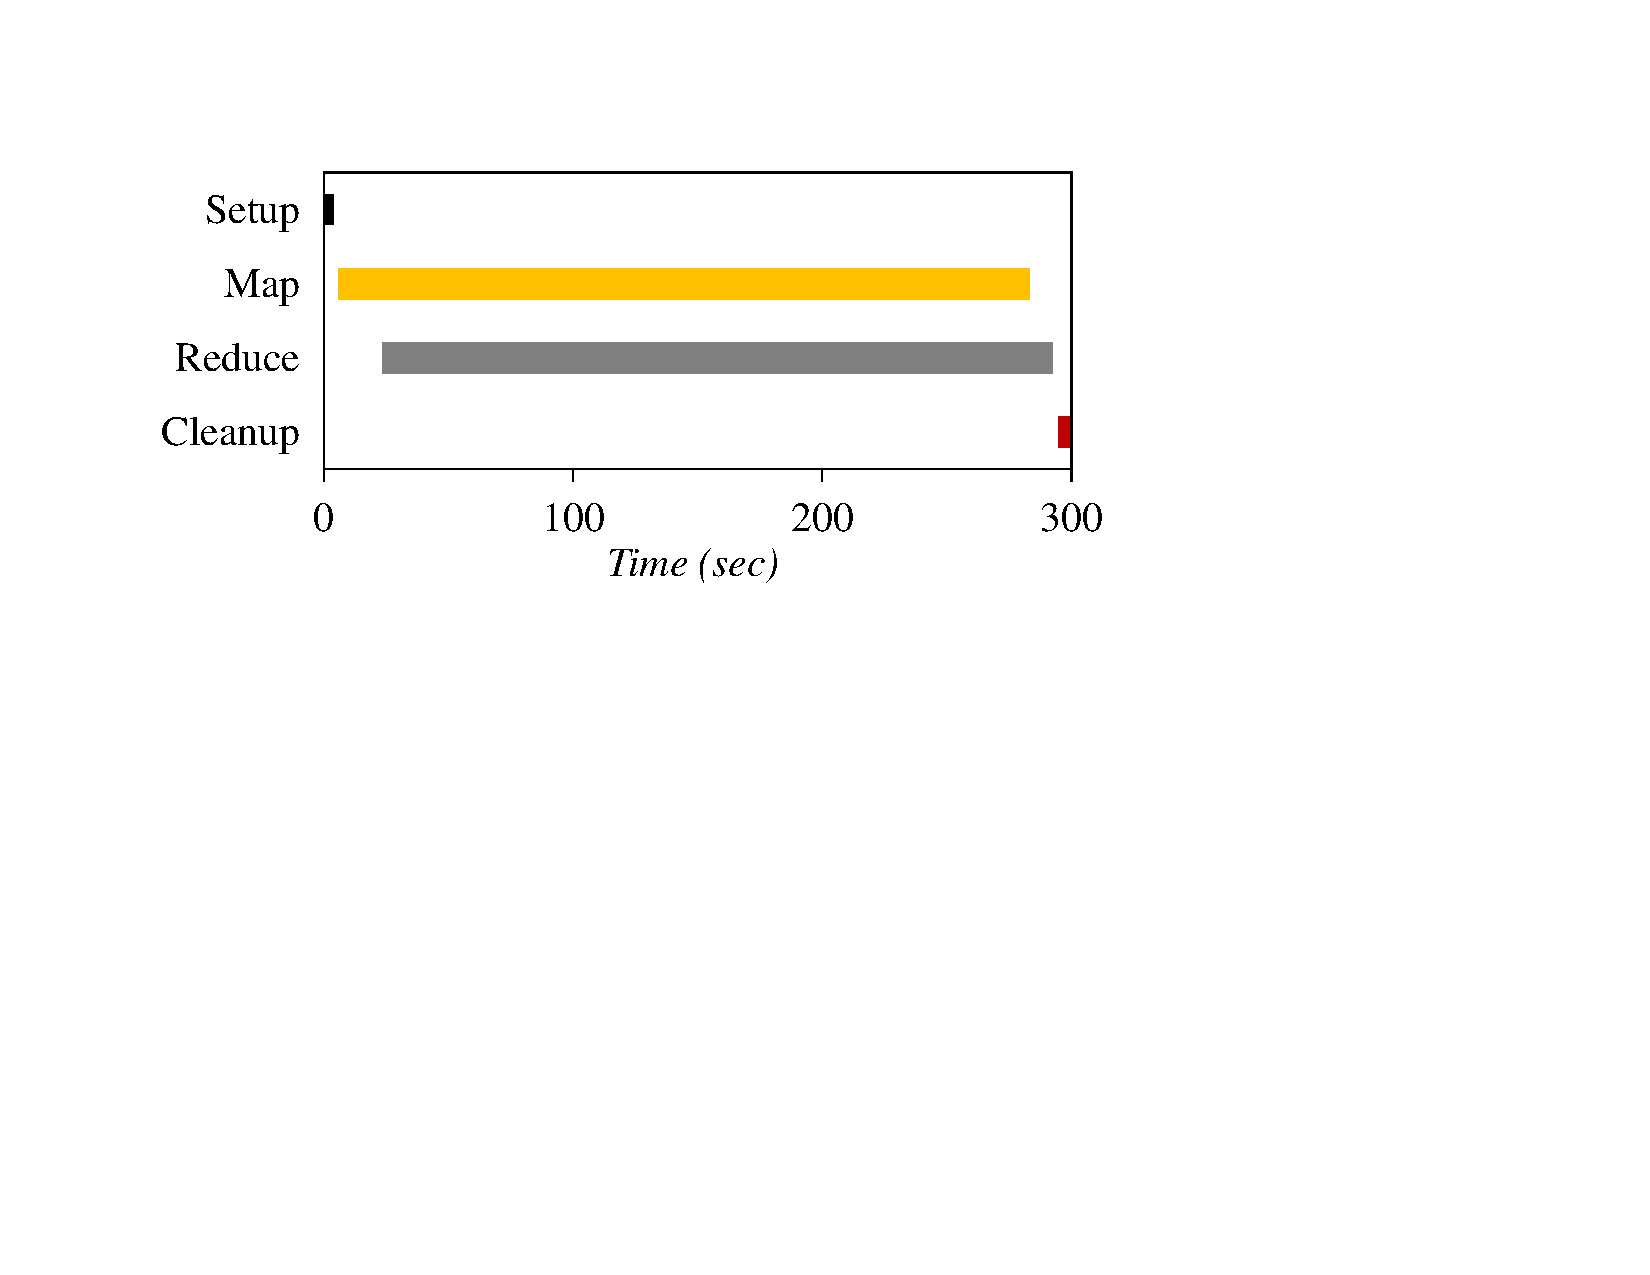
\includegraphics[width=0.8\columnwidth]{figures/Hadoop_execution_time_each_phase_breakdown1.pdf}
%	\caption{Total elapsed time breakdown of each phase}
%	\label{fig:Hadoop_total_time_BreakDown}
%\end{figure}


Figure~\ref{fig:time_breakdown} (b) makes a deeper analysis of the Hadoop task execution time. This figure shows the elapsed time of each Hadoop phase per each task. Each Hadoop task is subdivided into Map task and Reduce task. As a matter of fact, Hadoop sets up a job (setup time) at the beginning and deletes all intermediate data (cleanup time) after the job completion. These two tasks are performed only one time respectively throughout the whole job execution. That is, the total execution time of Hadoop application can be largely composed of one-time job setup time, many (depending on a data size) Map and Reduce tasks execution time, and one-time cleanup time. Considering this fact, Mapper execution time is a dominant factor of a total Hadoop execution time in wordcount-like Hadoop application. Based on these observations, our proposed ISC Hadoop framework moves Mapper to our ISC devices to improve Hadoop performance. As shown in Figure~\ref{fig:time_breakdown} (b), our ISC Hadoop system improves the Map task execution time by 2.5$\times$ faster (from 15 seconds to 6 seconds). All of our performance gain stems from this Mapper improvement.  


%\begin{figure}[htbp]
%	\centering
%		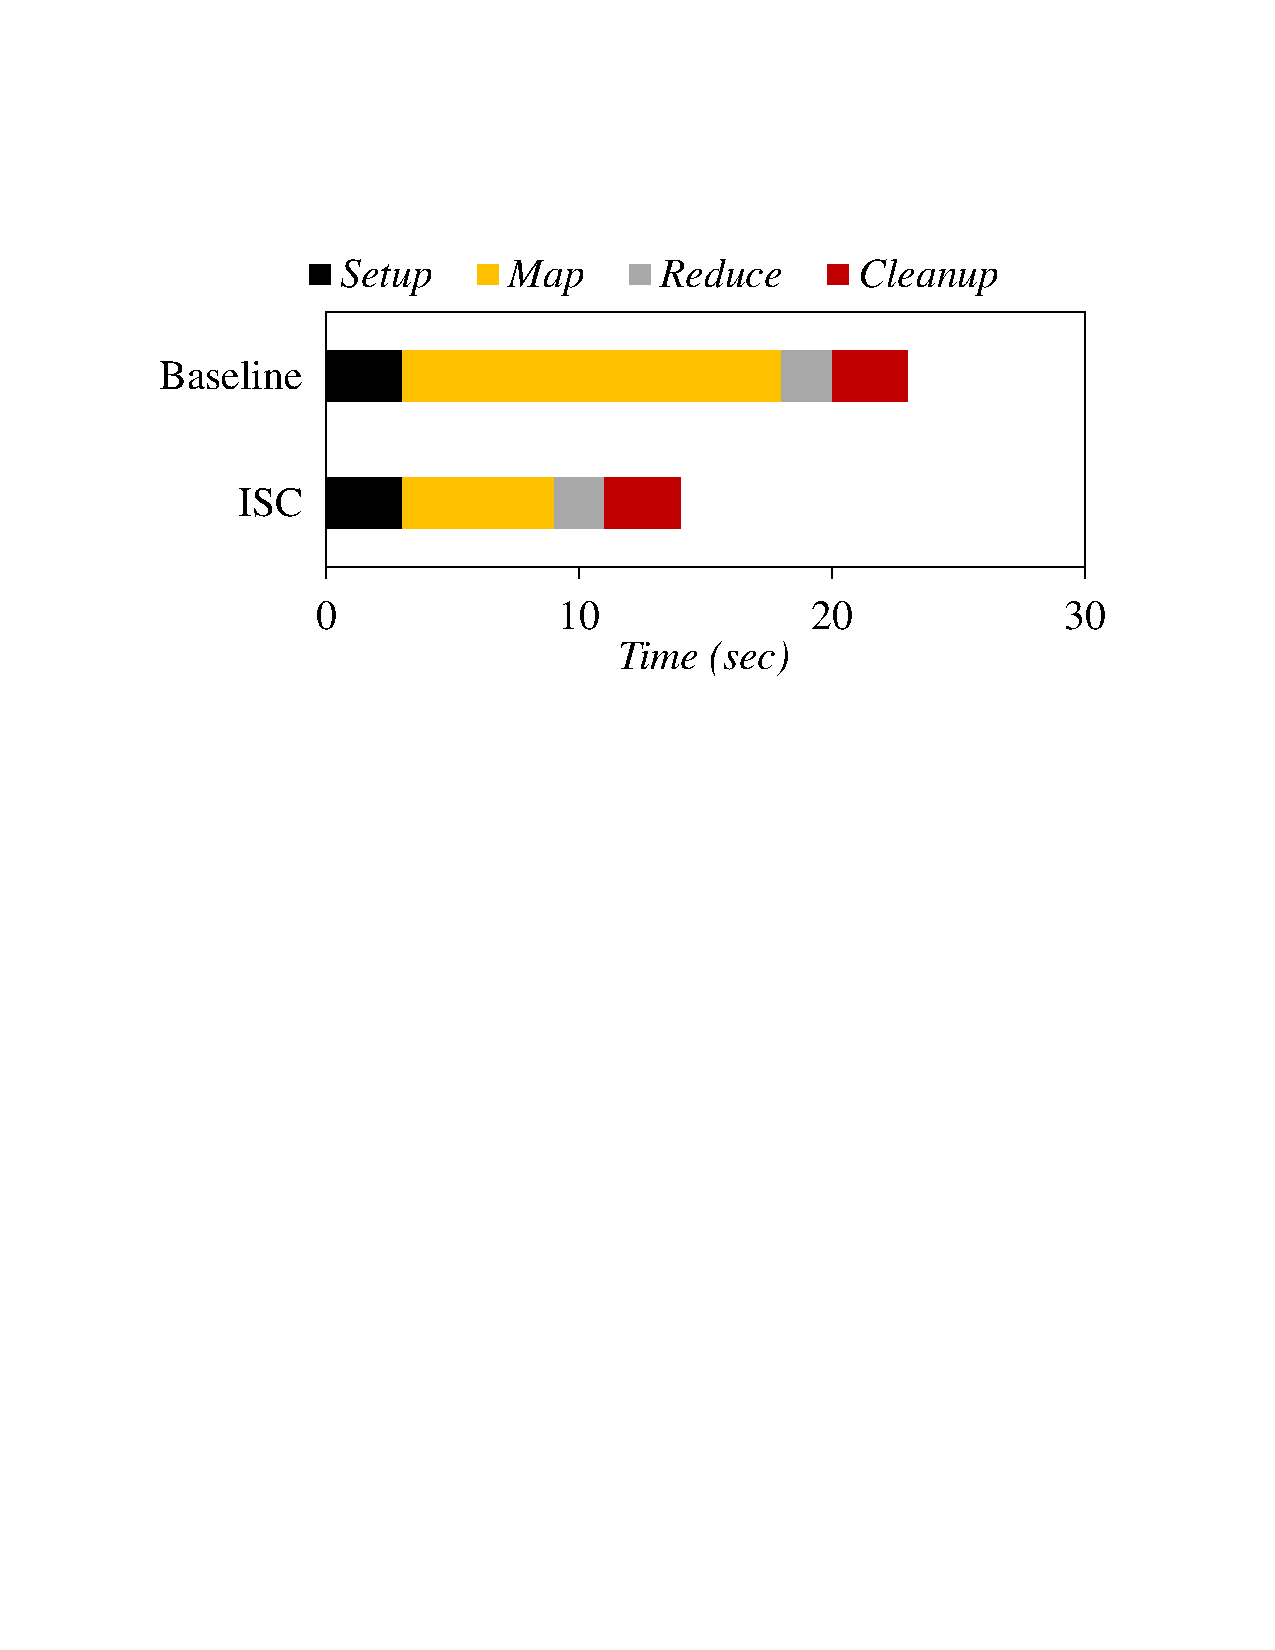
\includegraphics[width=0.8\columnwidth]{figures/Hadoop_time_breakdown.pdf}
%	\caption{Elapsed time breakdown per Hadoop task. Note: both setup and cleanup time here are one-time task per job, not per task.}
%	\label{fig:Hadoop_timeBreakDown}
%\end{figure}



Figure~\ref{fig:time_breakdown} (c) provides a even deeper analysis of the Mapper execution time. This plot corresponds to Map task execution time (i.e., yellow bar) in the Figure~\ref{fig:time_breakdown} (b). Similarly, Map task execution time is subdivided further into three elements: Map task setup time, Map task execution time, and Map task cleanup time. Both Map task setup time and cleanup time are almost constant time (in total 1.2 seconds). Thus, if we compare a \emph{pure} Map task execution time (i.e., yellow bar in the Figure~\ref{fig:time_breakdown}) (c) between them, our performance gain is even larger (3.6$\times$). However, each Map task requires such extra constant time (i.e., both Map task setup time and cleaning time, about 2--3 sec/Map) as well as Map task execution time. This constant time is relatively big portion (about 36\%) to Map task in ISC Hadoop system, compared to the portion (14.6\%) in baseline. Therefore, this larger performance gain (3.6$\times$) is lessened to 2.5$\times$ in Figure~\ref{fig:time_breakdown} (b), and similarly to 2$\times$ in end-to-end total execution time (Figure~\ref{fig:execution_time_with_single_namenode_on_single_node}).


%\begin{figure}[htbp]
%	\centering
%		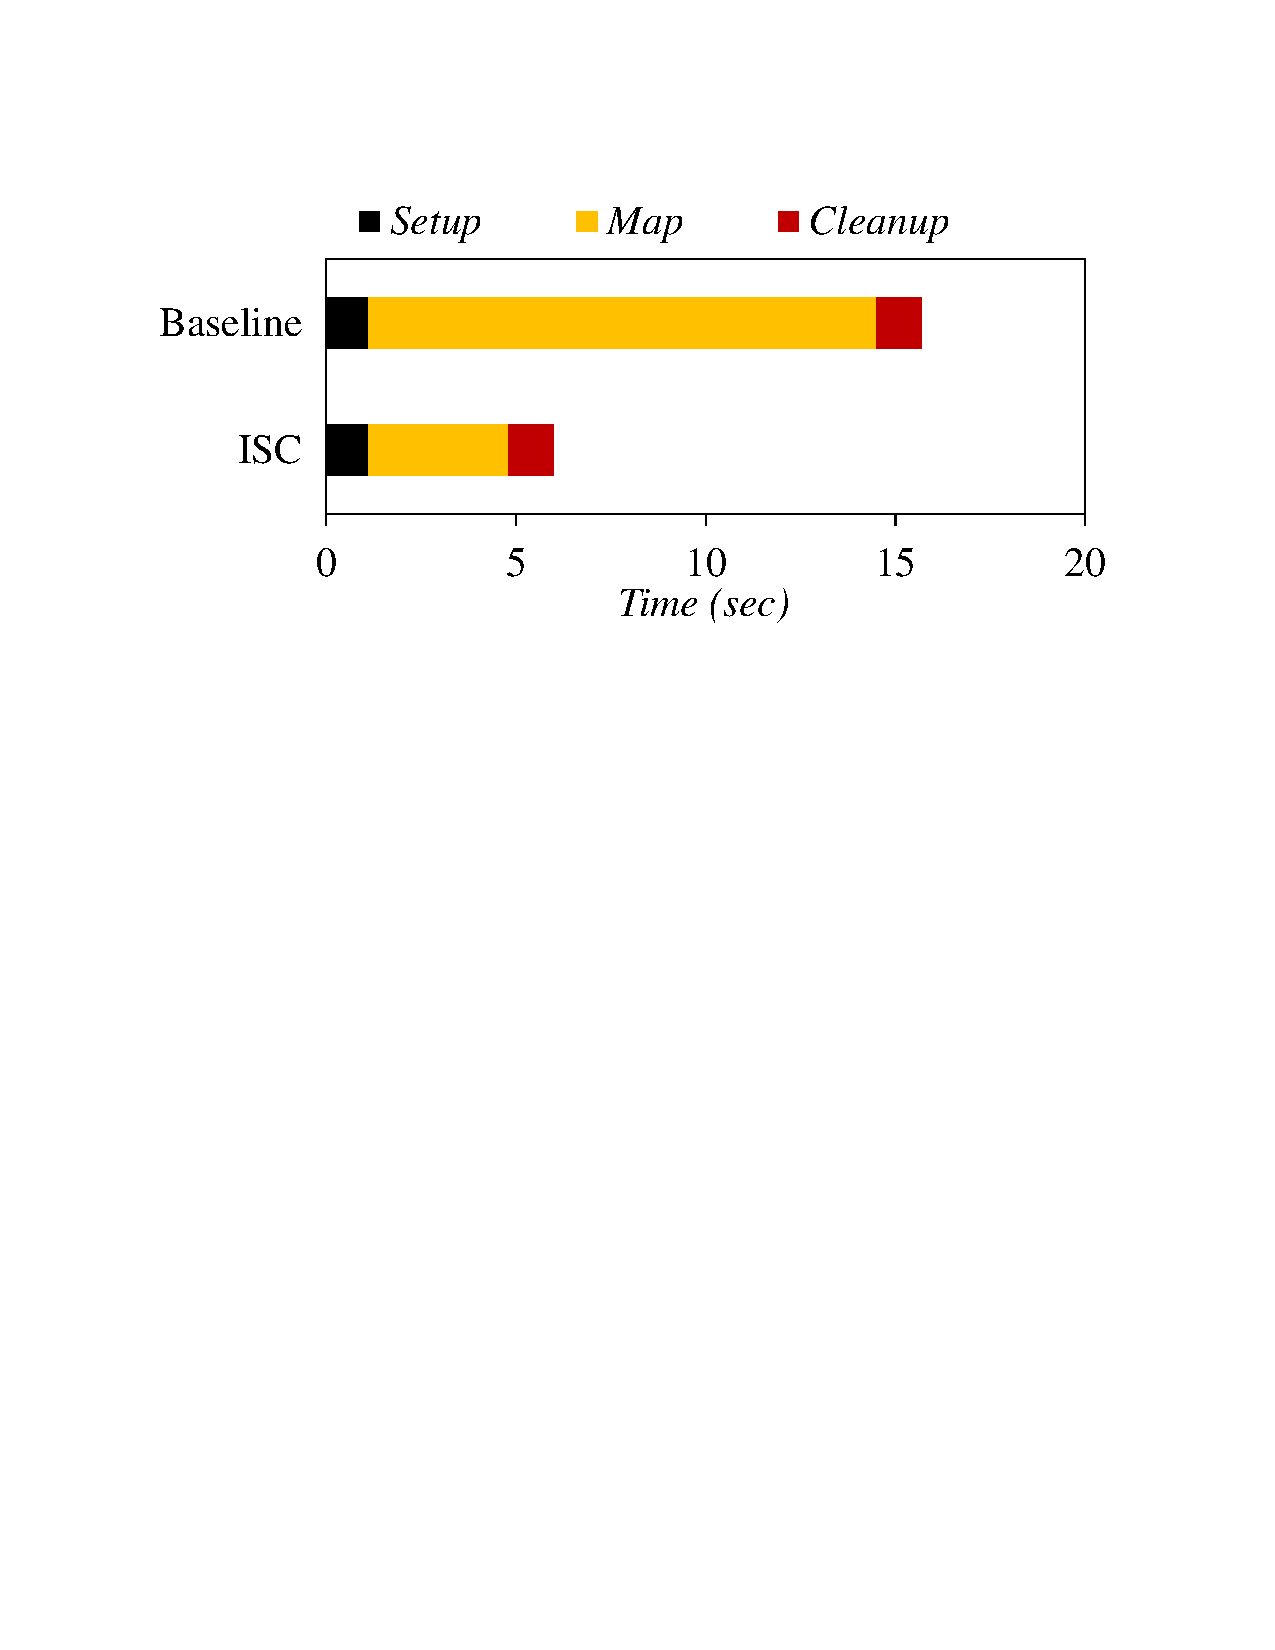
\includegraphics[width=0.8\columnwidth]{figures/Hadoop_breakdown_per_maptask.pdf}
%	\caption{Elapsed time breakdown per Map task}
%	\label{fig:Hadoop_timeBreakDown_per_mapTask}
%\end{figure}



\begin{figure}[htbp]
  \centering
  \renewcommand{\tabcolsep}{0.1mm}
  \begin{tabular}{ccc}
 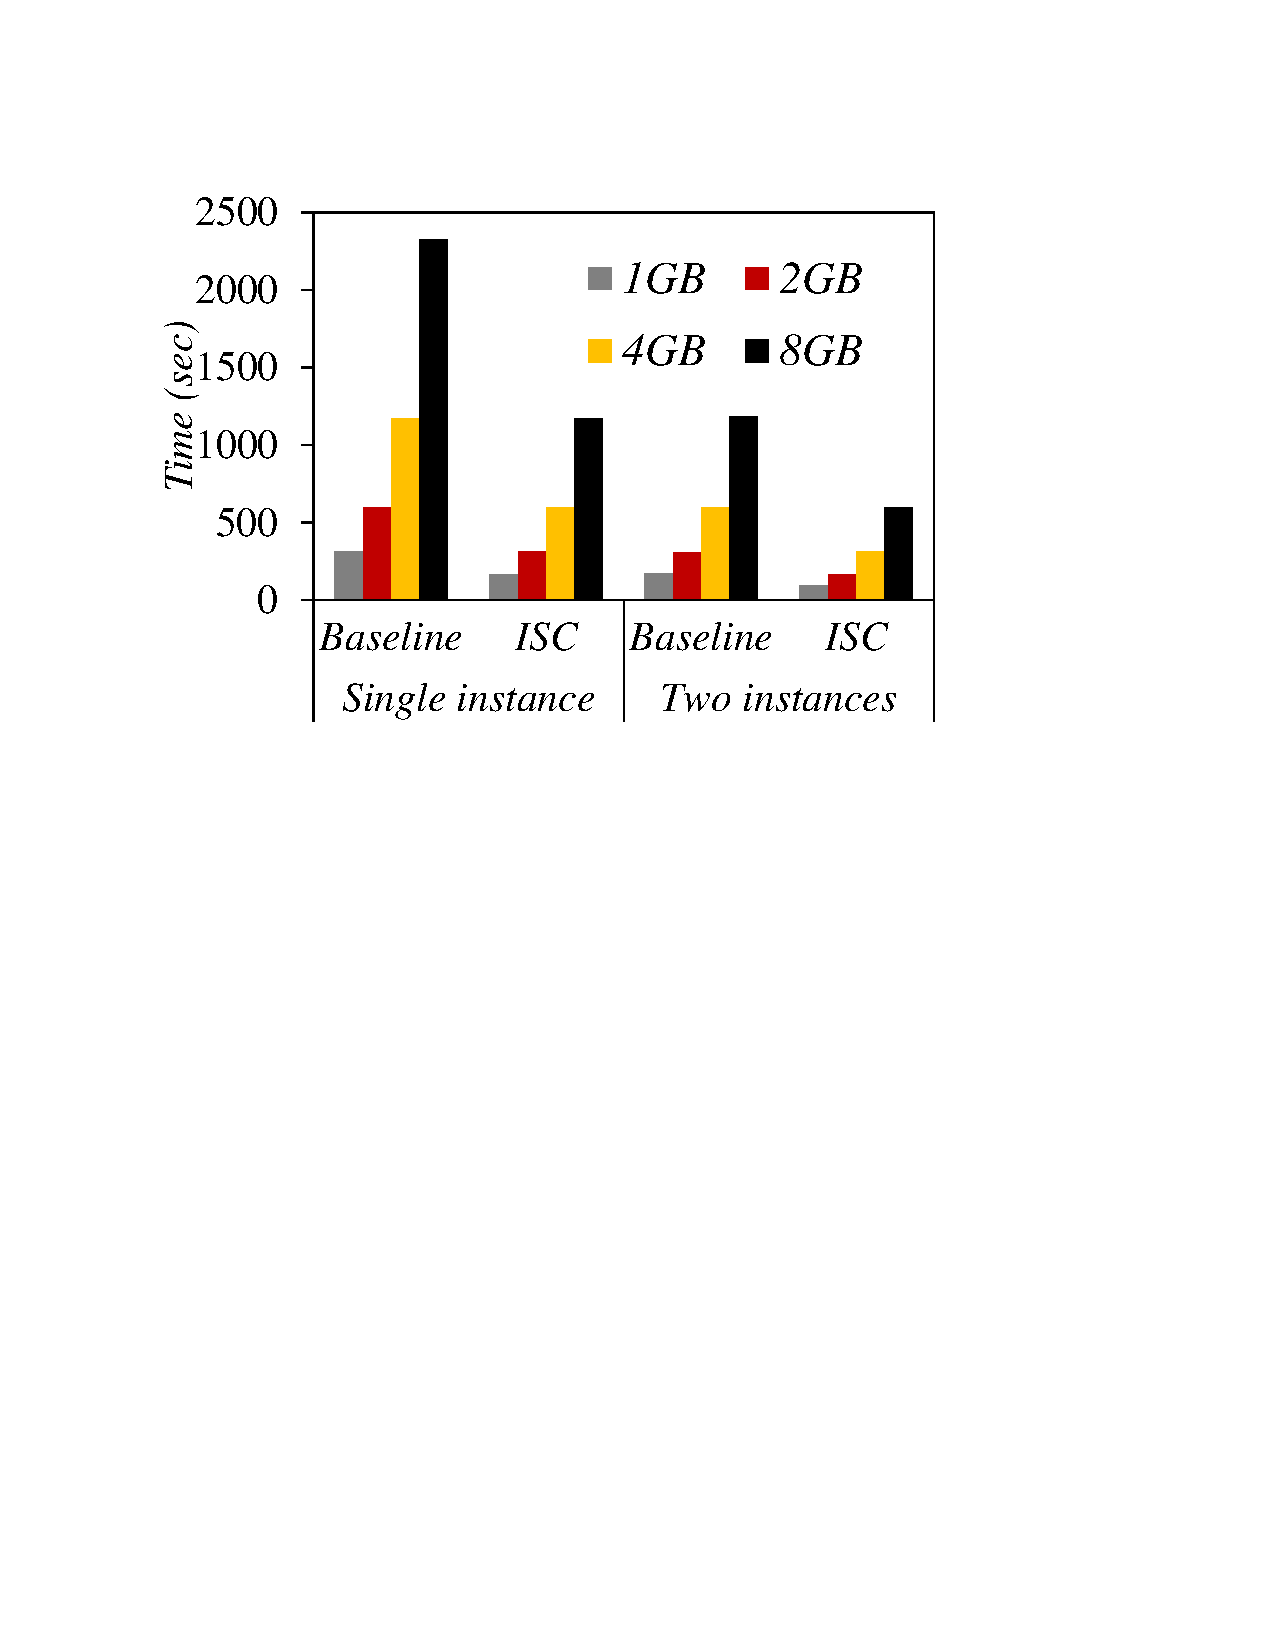
\includegraphics[width=0.5\columnwidth]{figures/Hadoop_total_execution_time_single_two_nodes.pdf}&
  %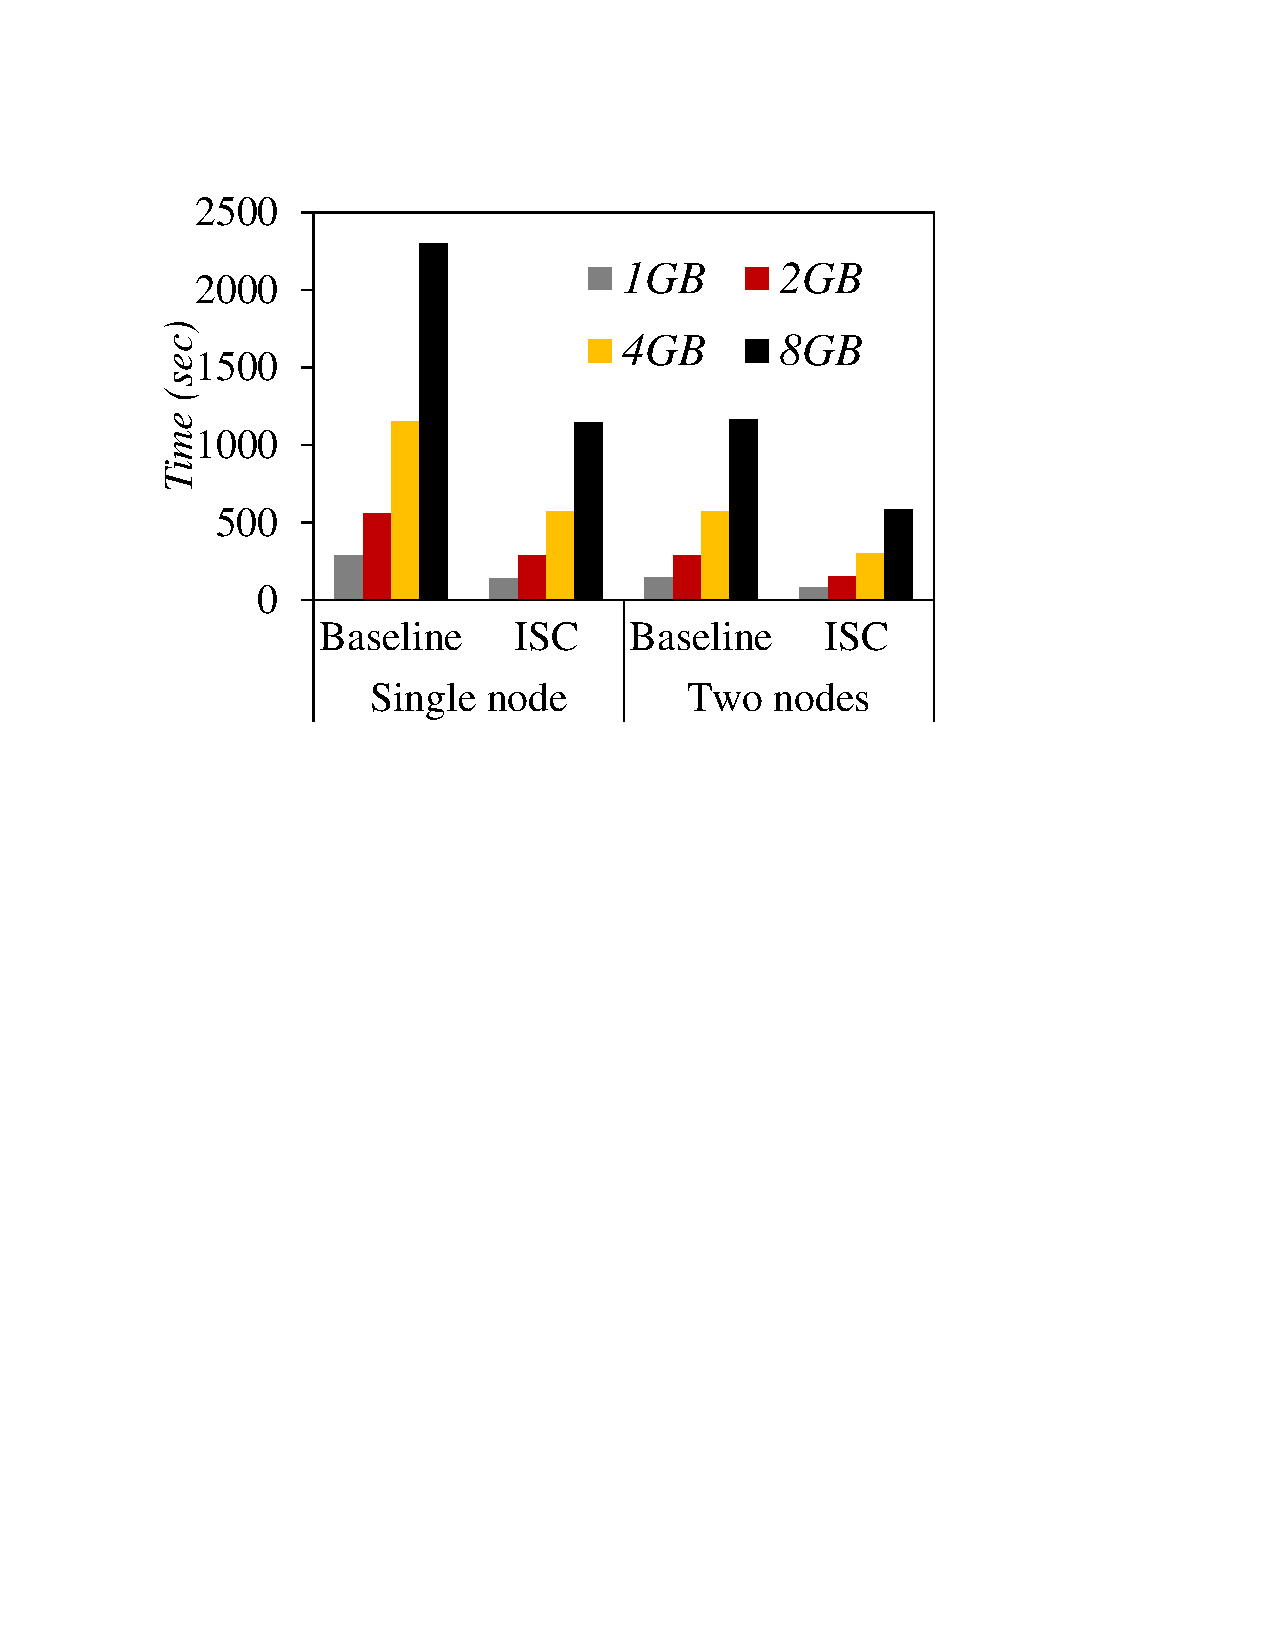
\includegraphics[width=0.5\columnwidth]{figures/Hadoop_mapper_execution_time_single_two_nodes.pdf}\\
  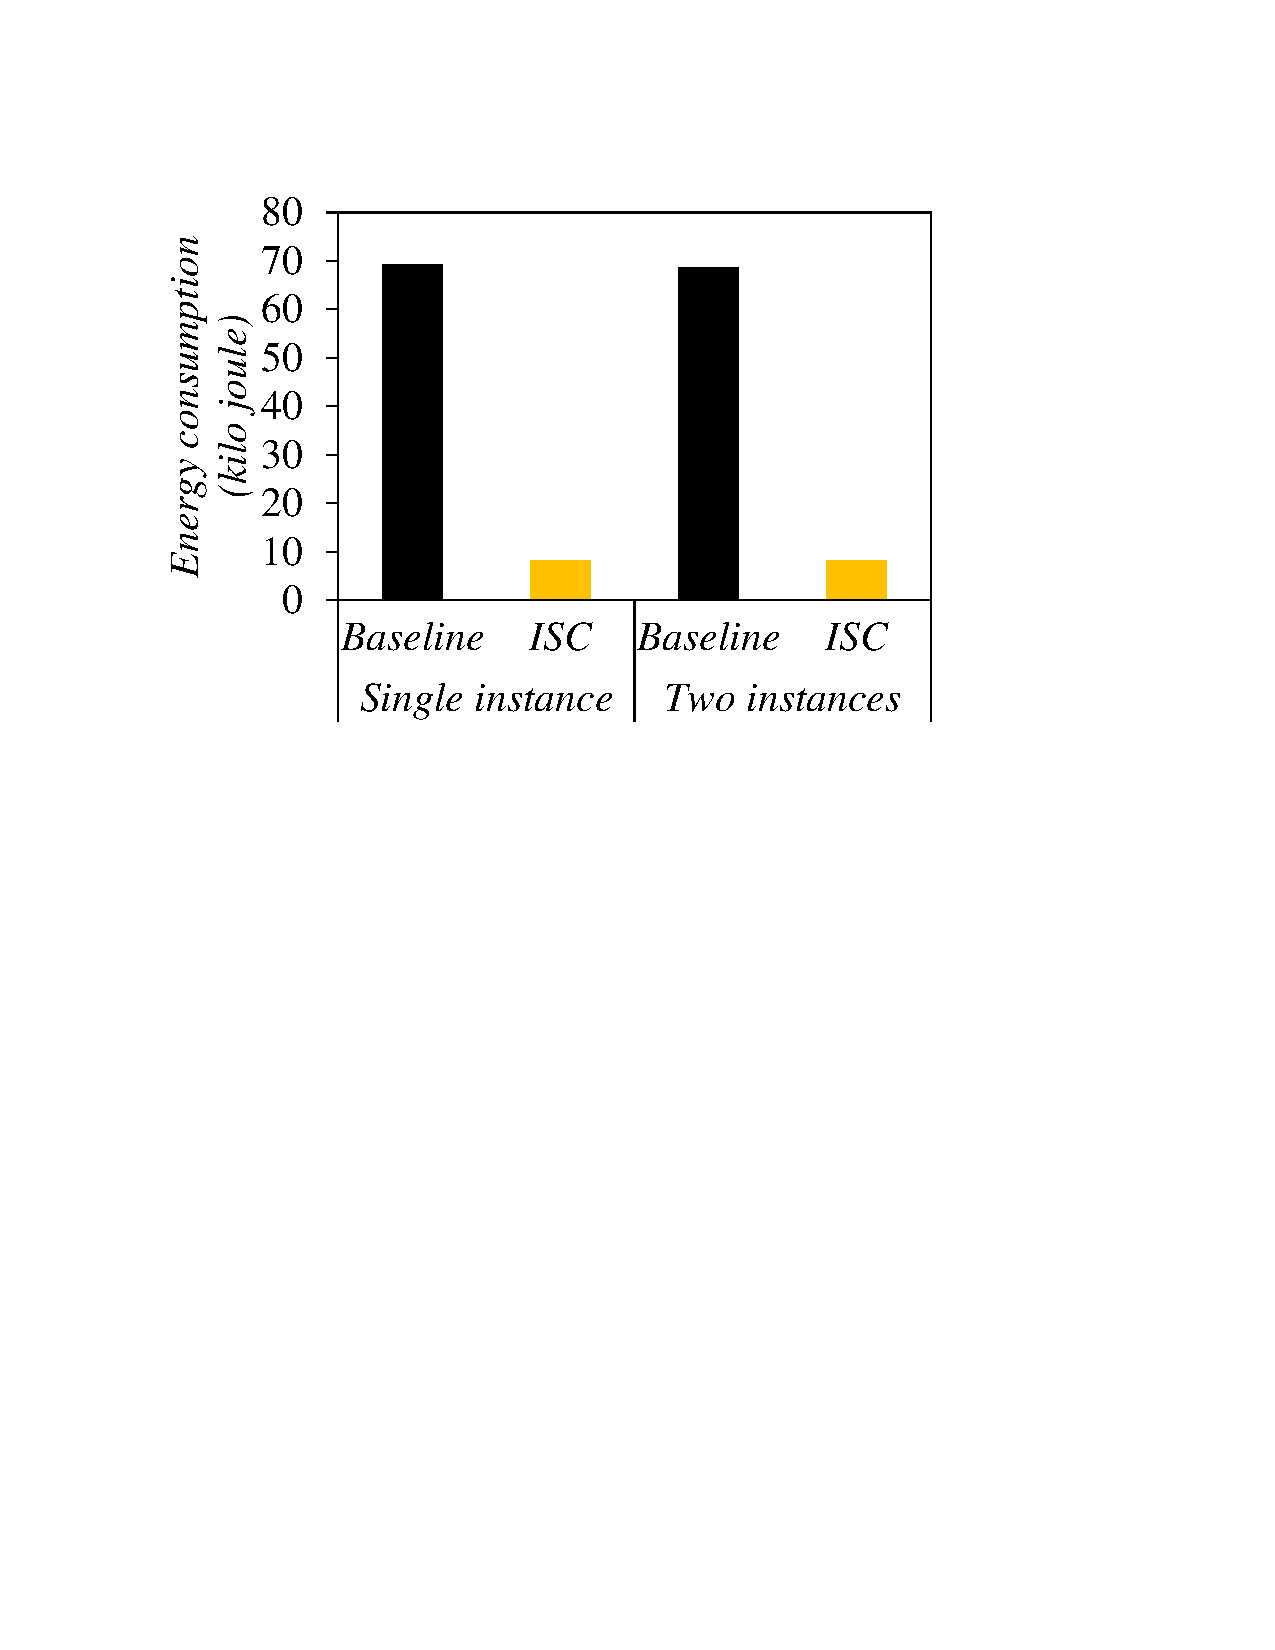
\includegraphics[width=0.5\columnwidth]{figures/Hadoop_power_consumption_single_node.pdf}\\	
  (a) Total Elapsed Time & (b) Total Energy Consumption
\end{tabular}
  \caption{Single instance vs. two instances on a single node}
  \label{fig:execution_time_with_two_namenode_on_single_node}
 \end{figure}




\begin{figure*}[t]
  \centering
  \renewcommand{\tabcolsep}{1mm}
  \begin{tabular}{ccc}
 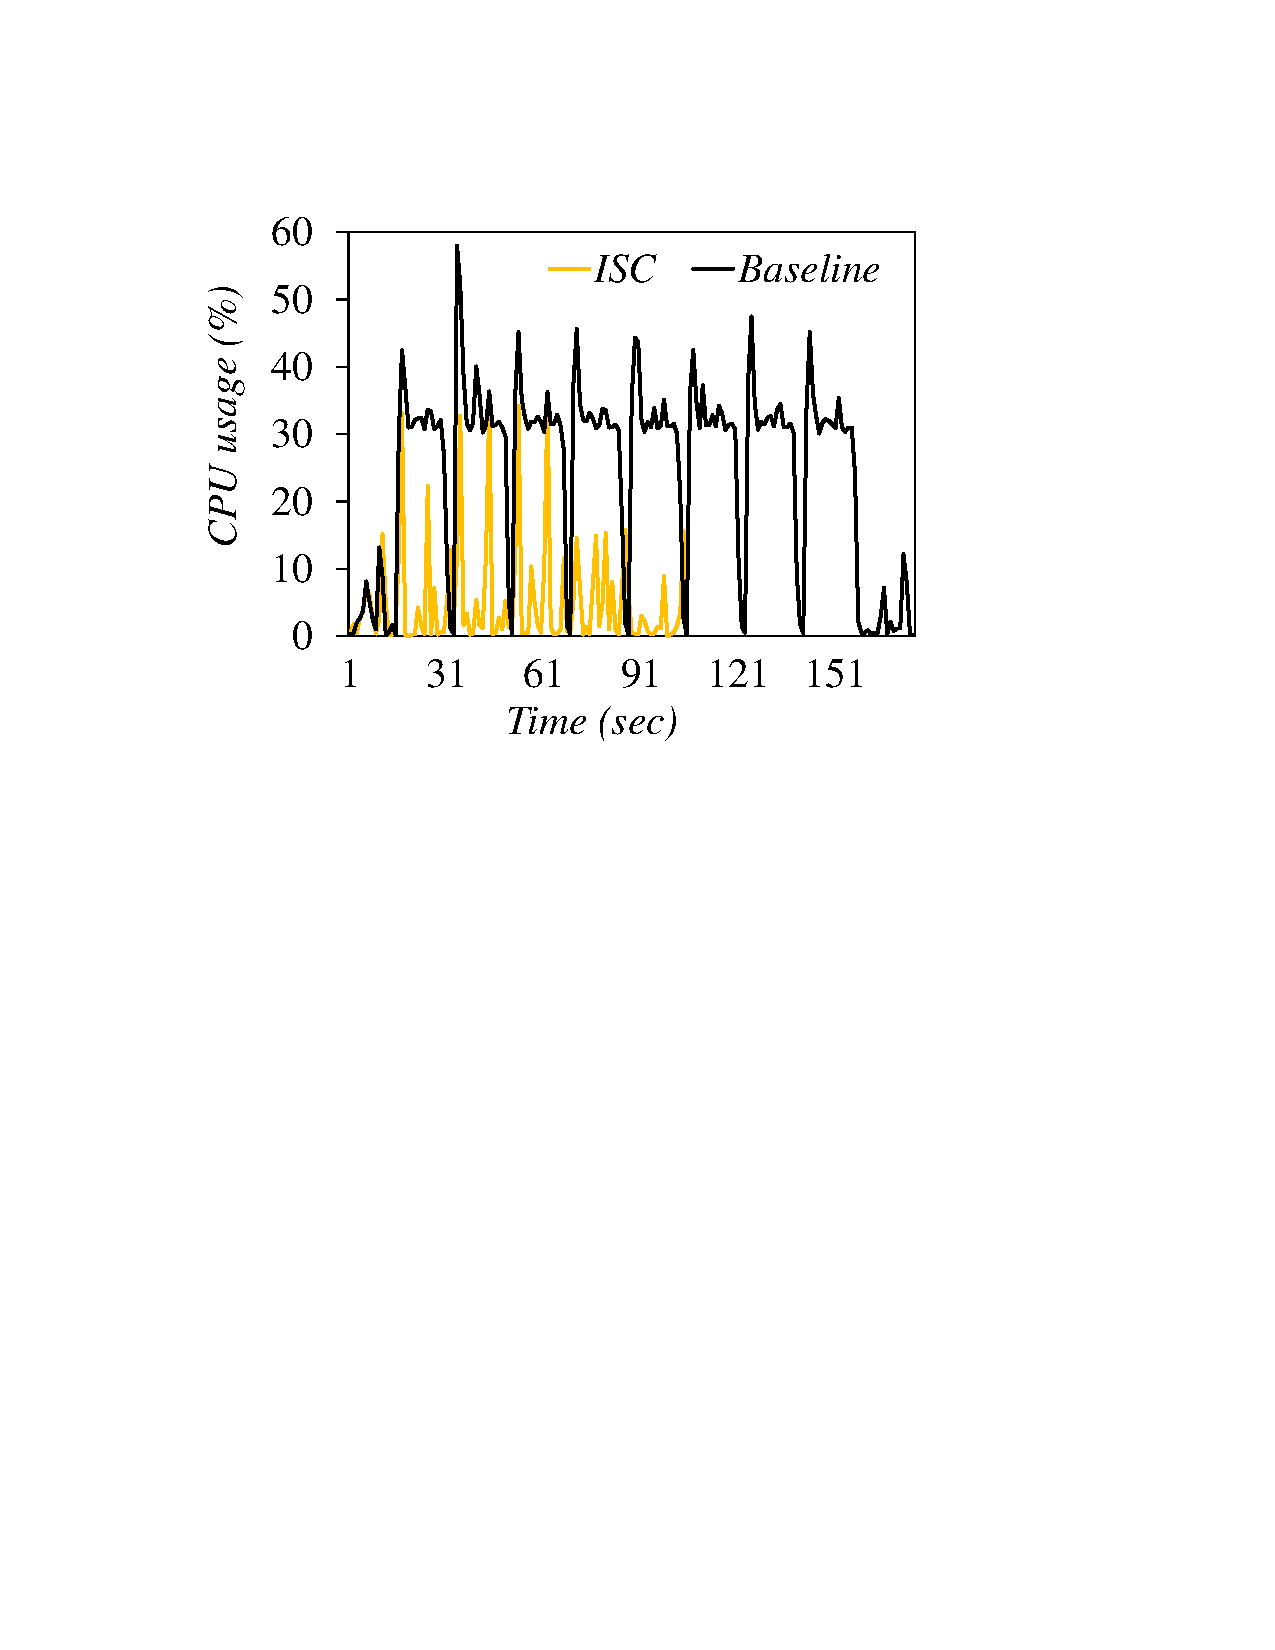
\includegraphics[width=0.66\columnwidth]{figures/Hadoop_CPU_usage.pdf}&
  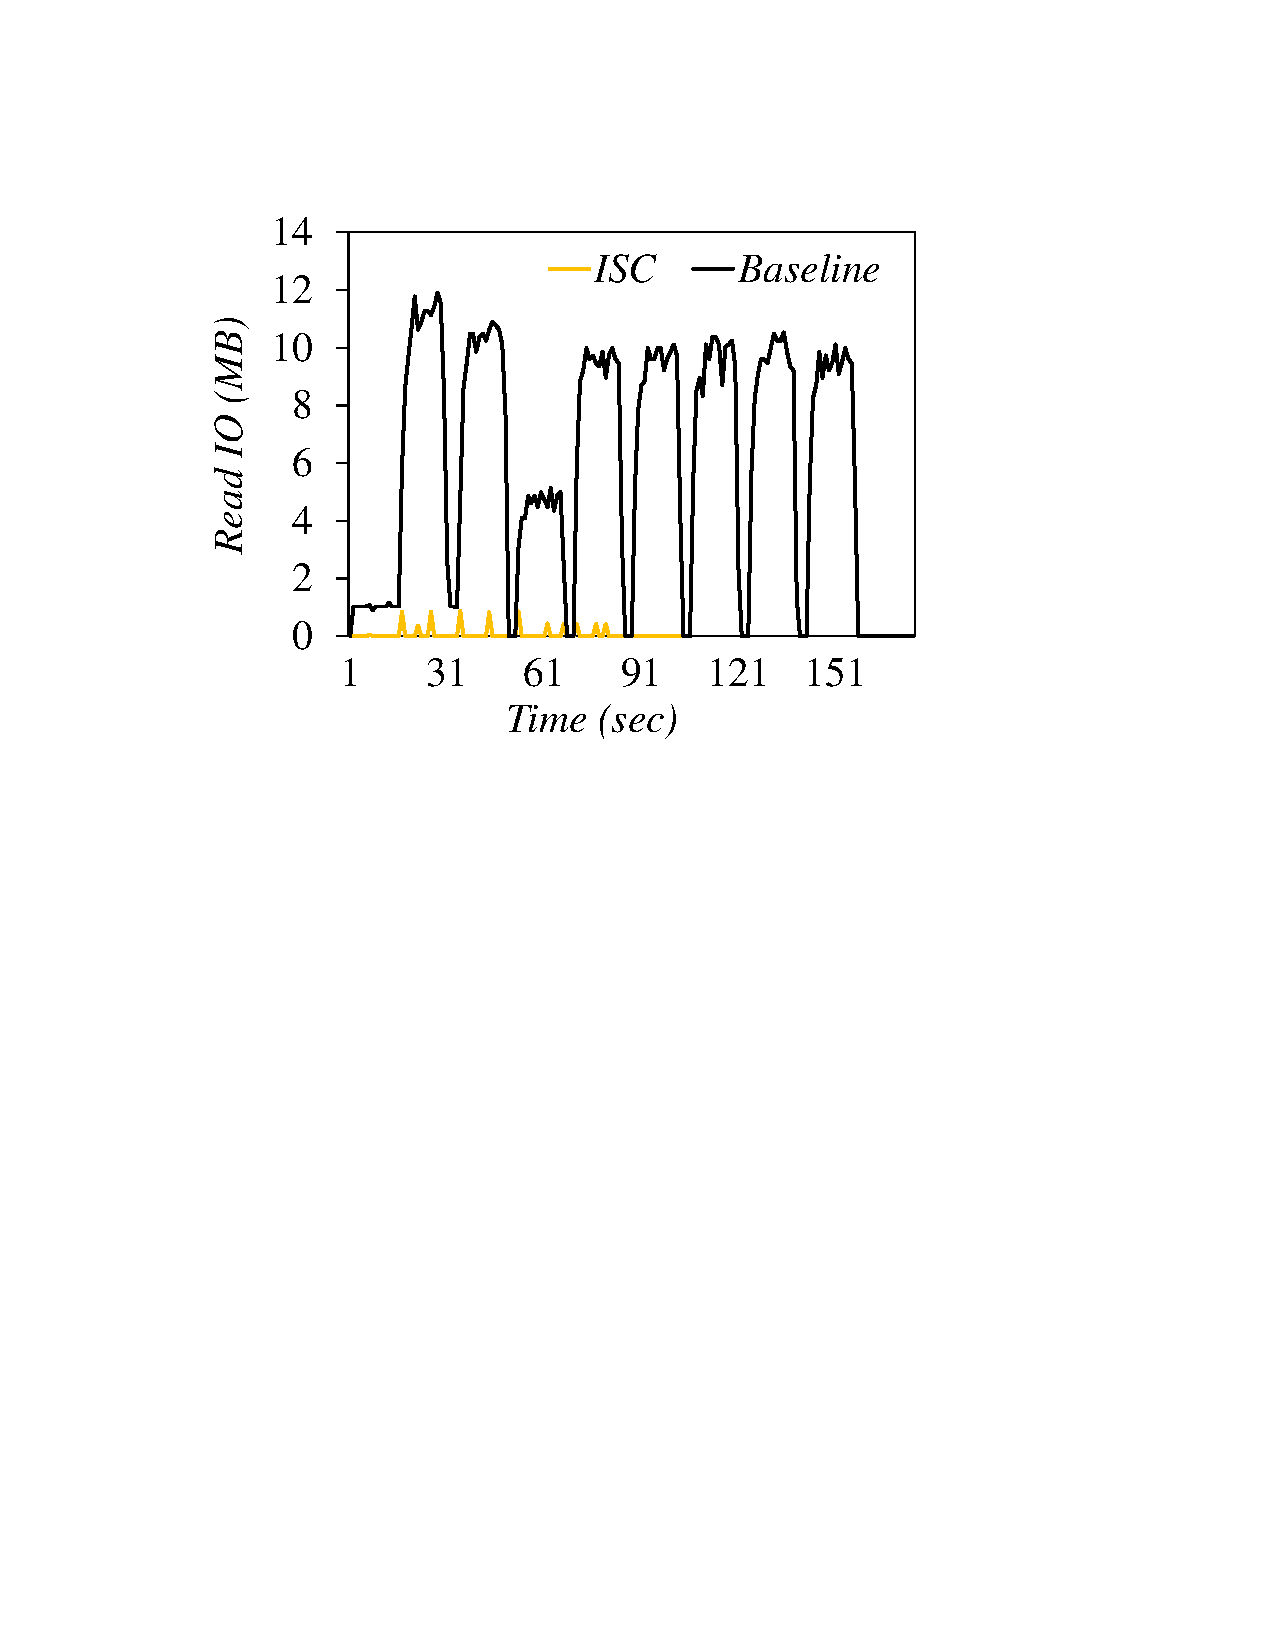
\includegraphics[width=0.66\columnwidth]{figures/Hadoop_read_io.pdf}&
  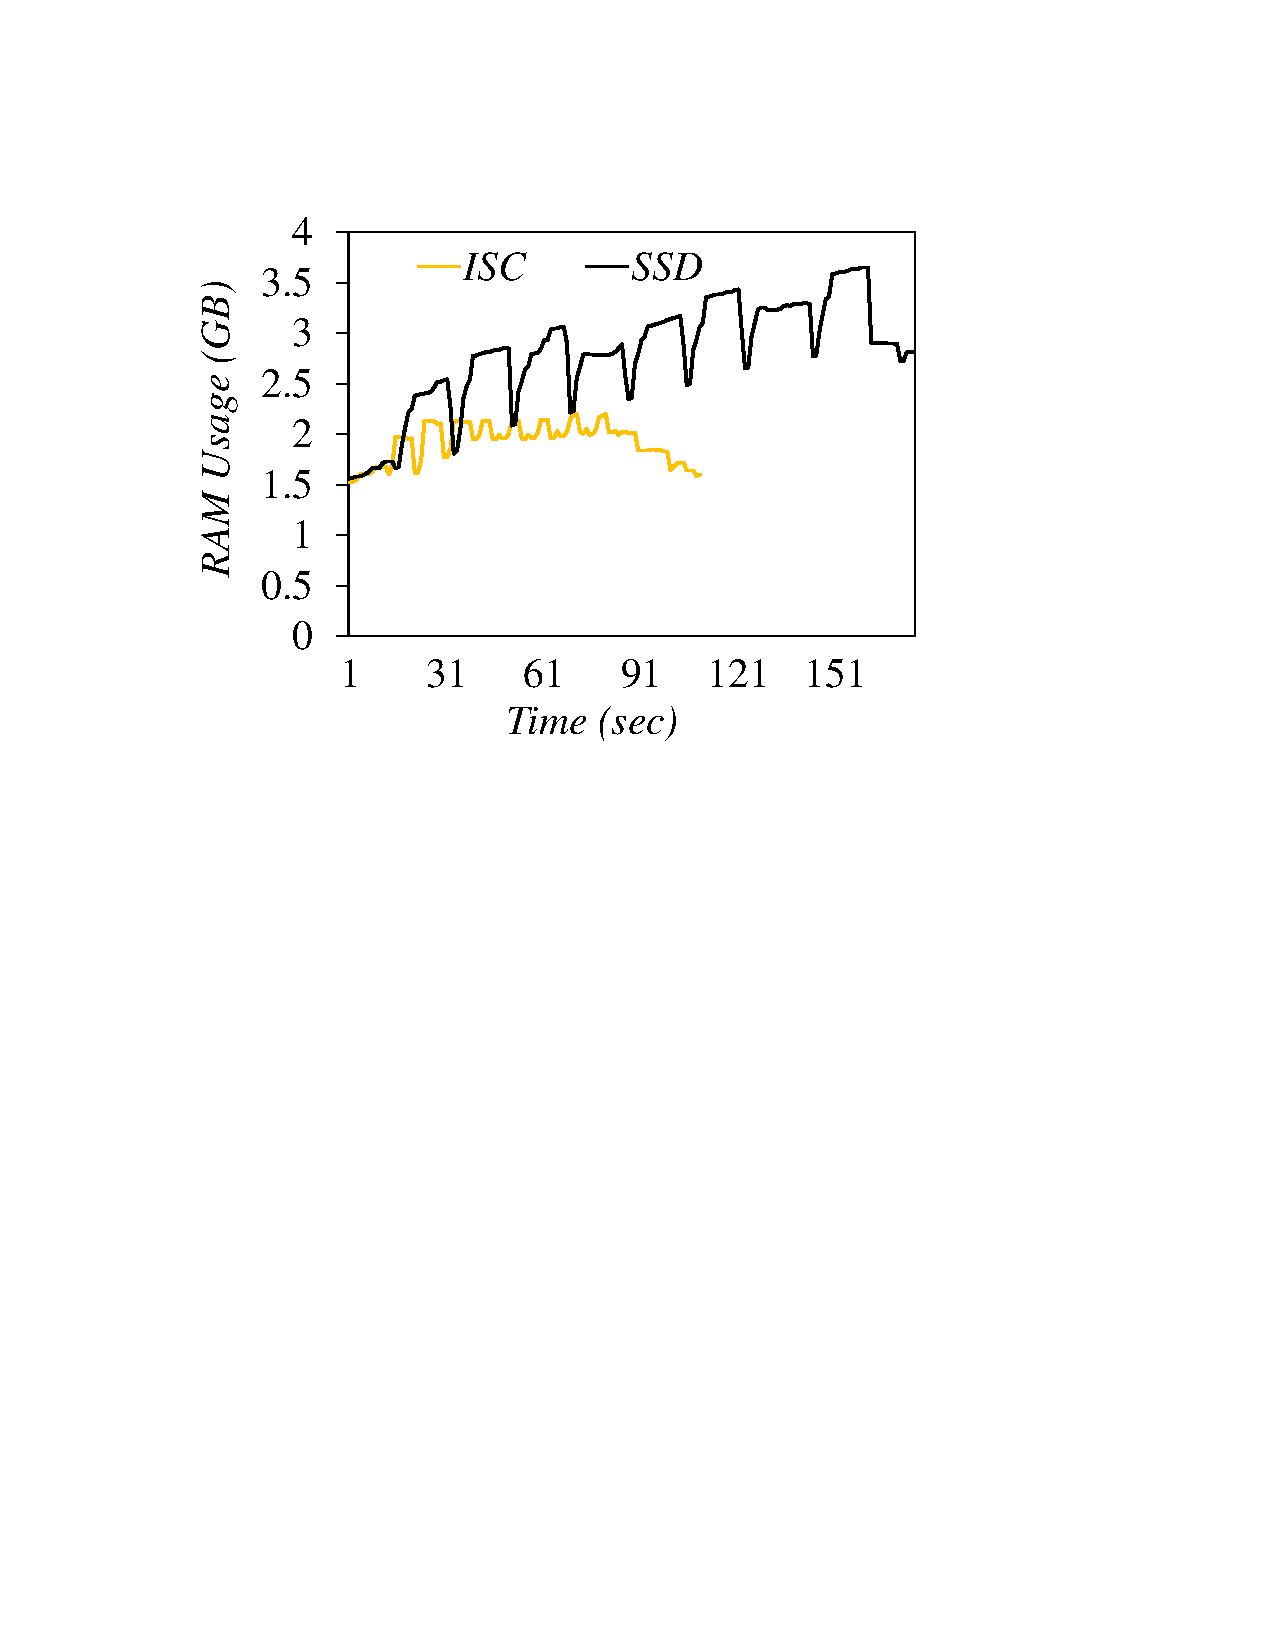
\includegraphics[width=0.66\columnwidth]{figures/Hadoop_RAM_usage.pdf}\\	
  (a) Host CPU Usage & (b) Host Read I/O & (c) Host DRAM Usage
\end{tabular}
  \caption{Host system resource usage}
  \label{fig:host_resource_usage}
\end{figure*}


\begin{figure*}[t]
  \centering
  \renewcommand{\tabcolsep}{1mm}
  \begin{tabular}{ccc}
 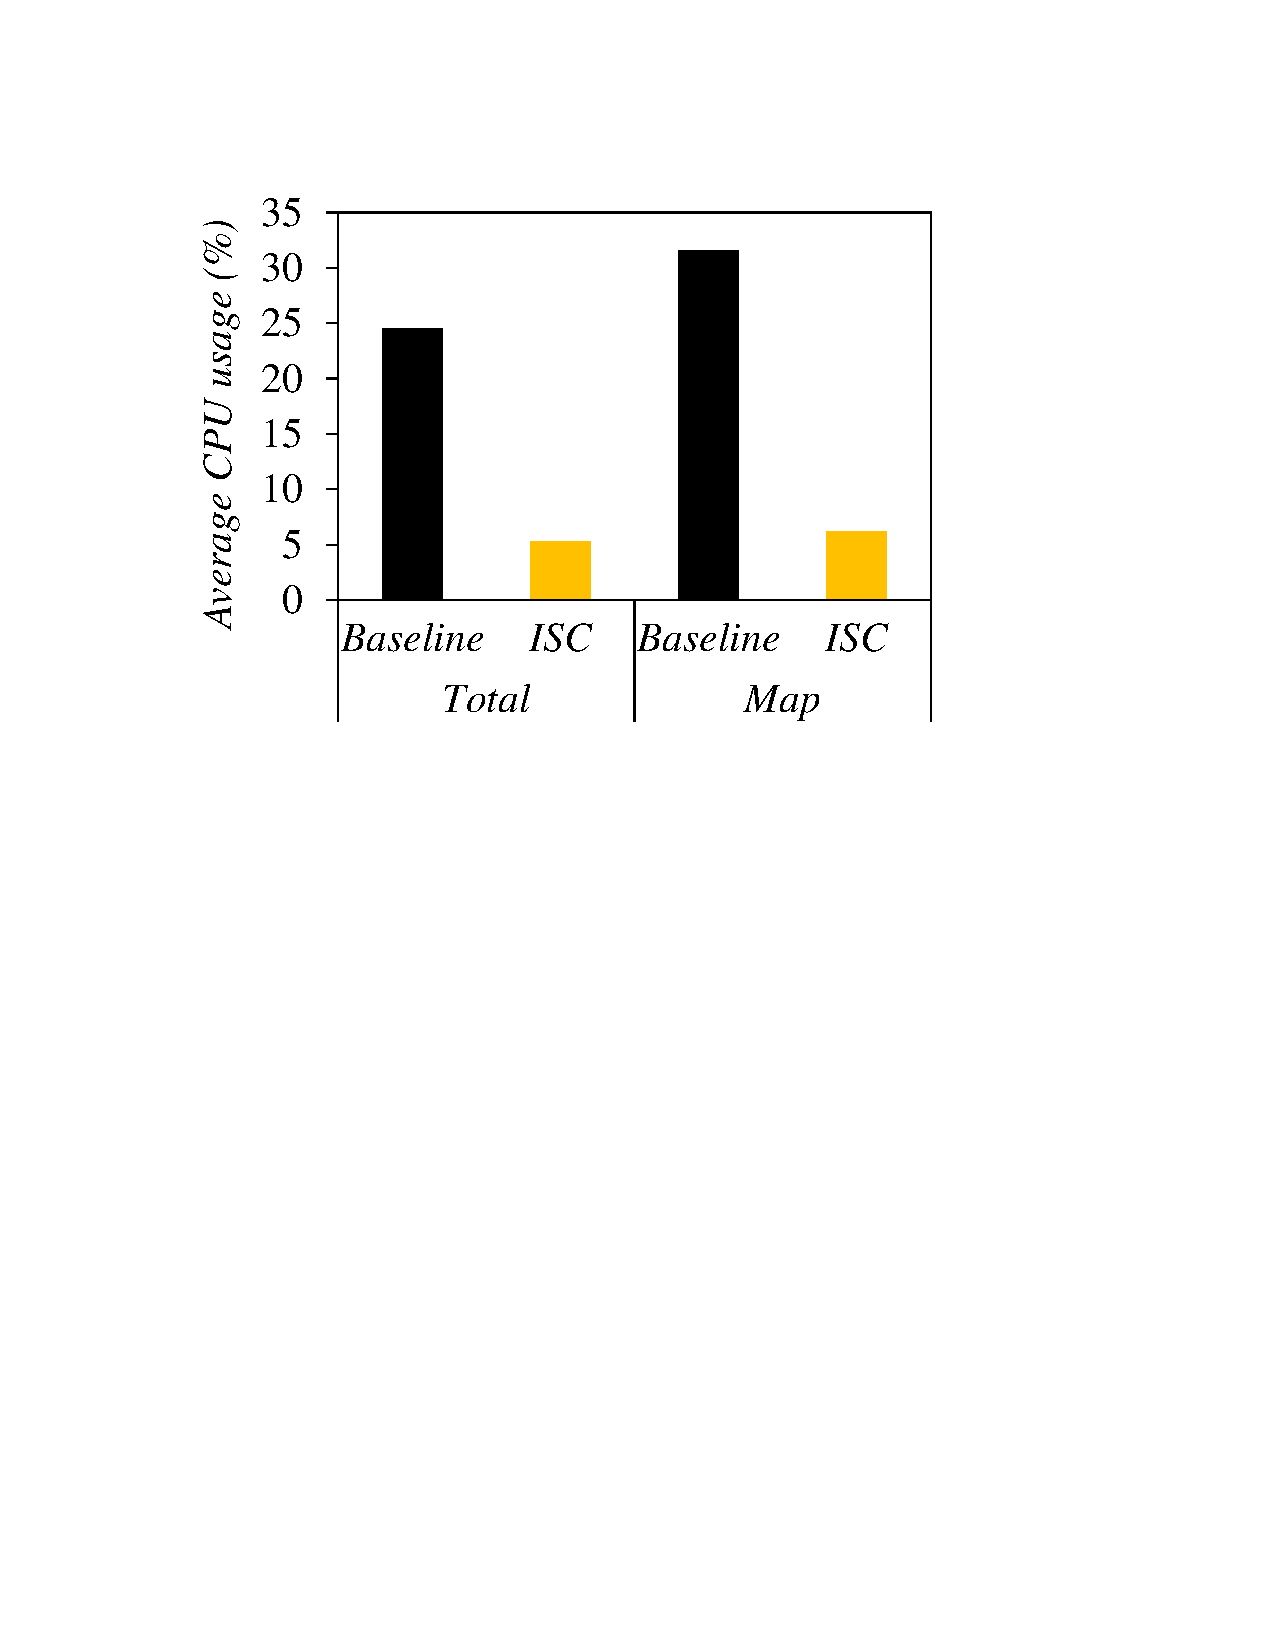
\includegraphics[width=0.66\columnwidth]{figures/Hadoop_average_CPU_usage.pdf}&
  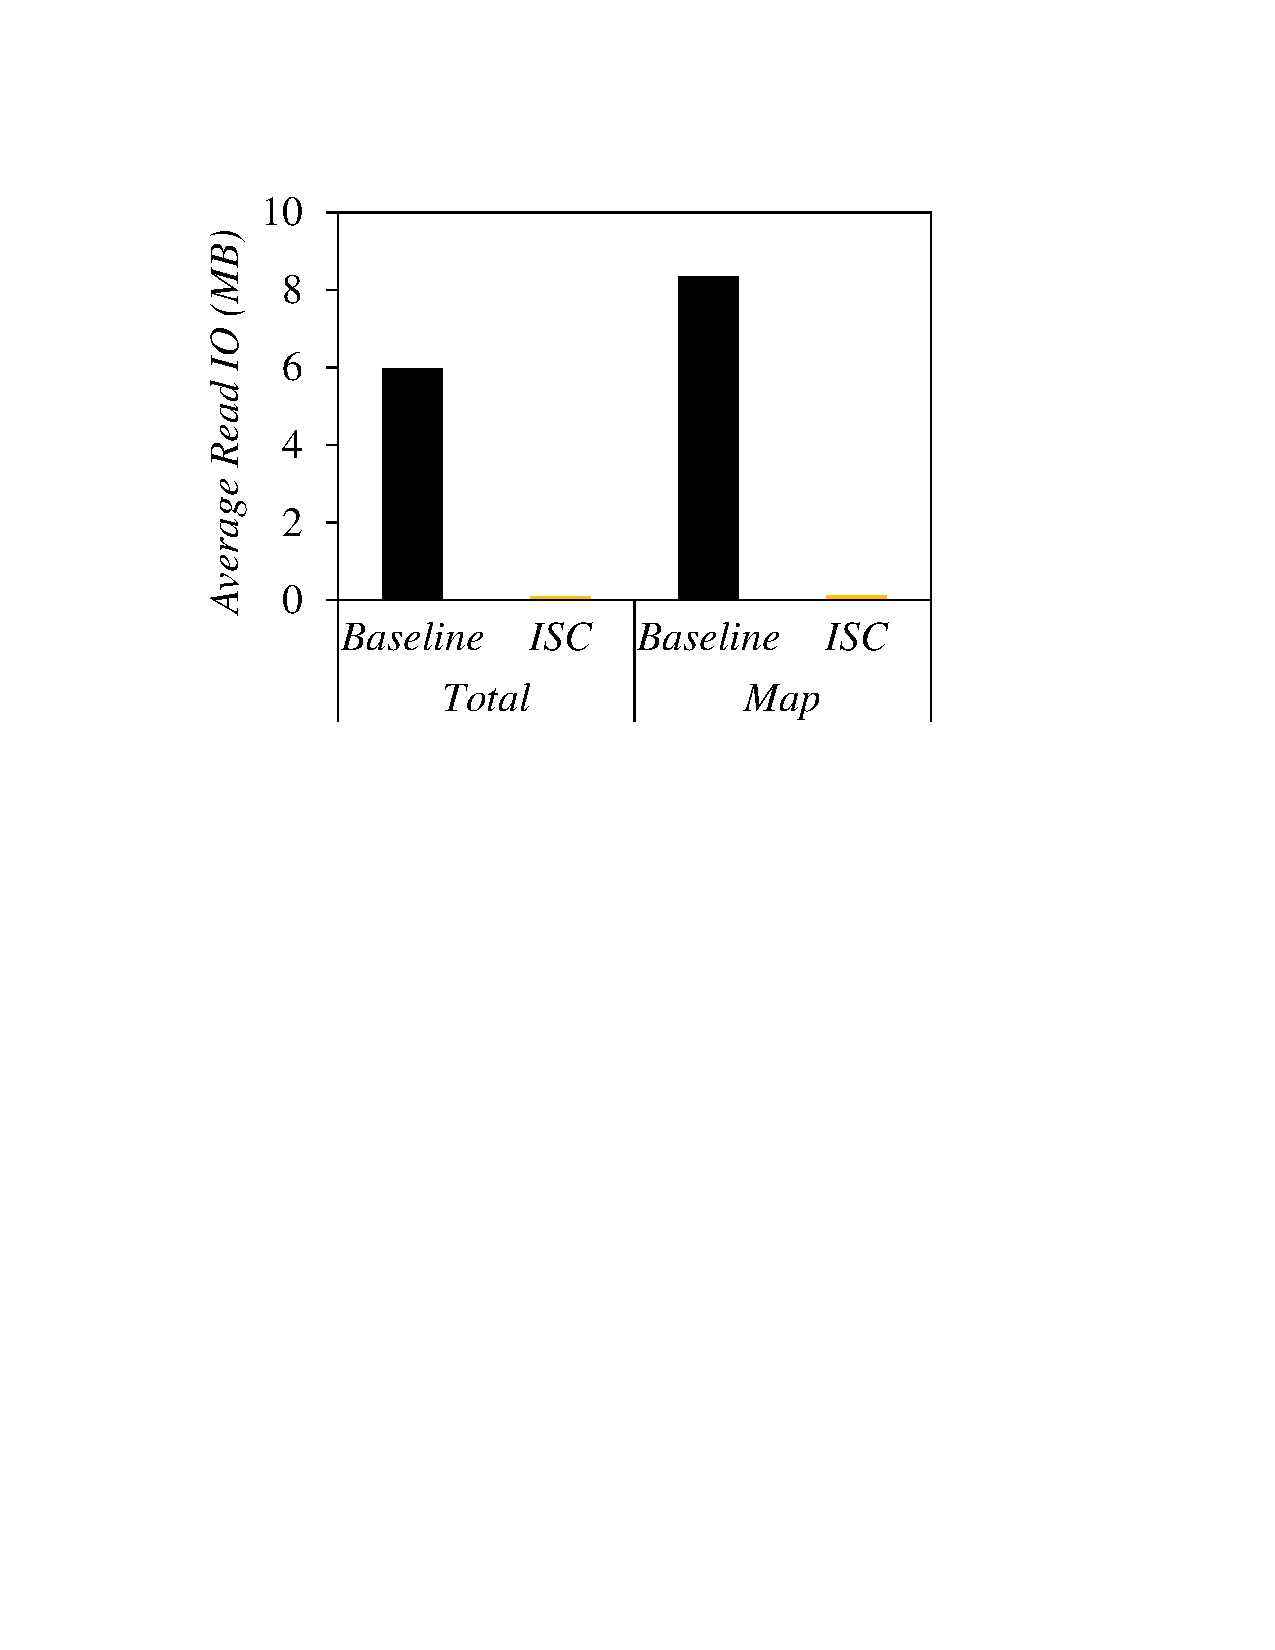
\includegraphics[width=0.66\columnwidth]{figures/Hadoop_average_read_io.pdf}&
  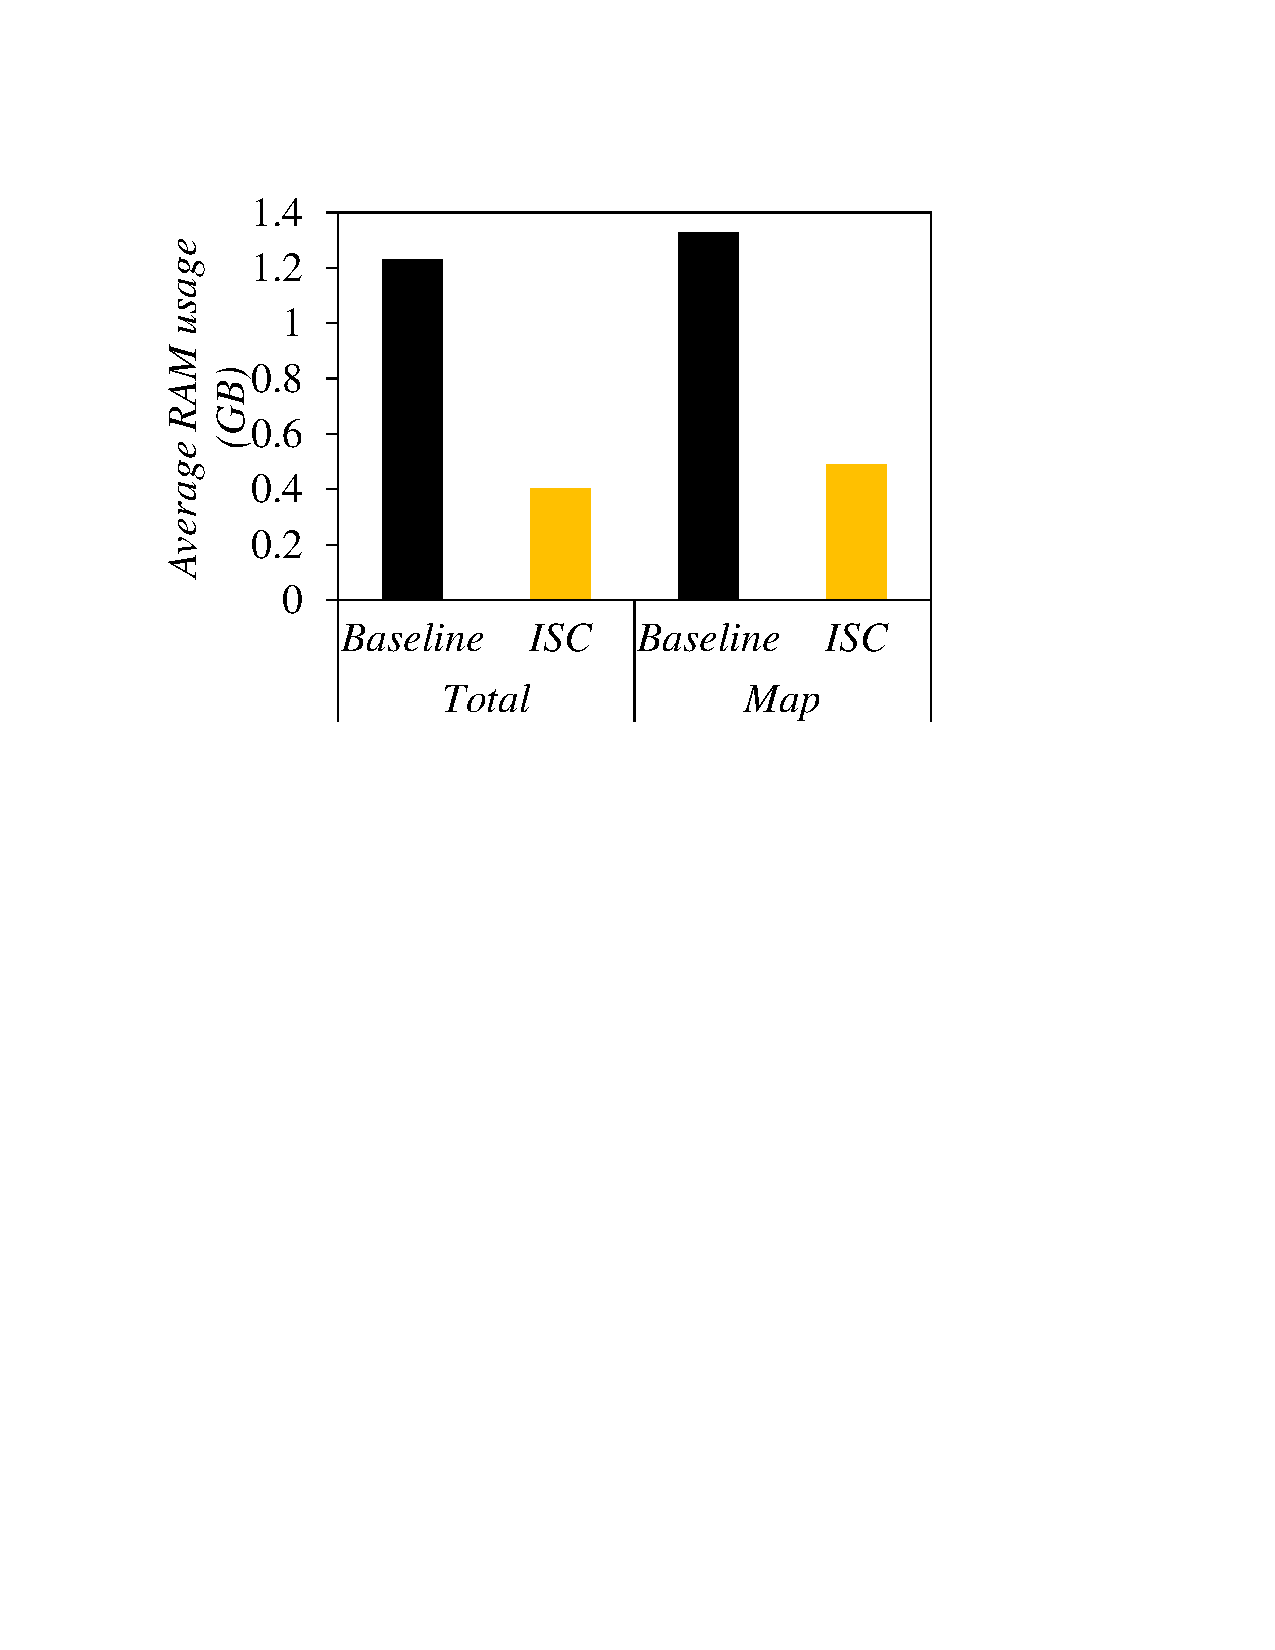
\includegraphics[width=0.66\columnwidth]{figures/Hadoop_average_RAM_usage.pdf}\\	
  (a) Average Host CPU Usage & (b) Average Host Read I/O & (c) Average Host DRAM Usage
\end{tabular}
  \caption{Average host system resource usage}
  \label{fig:avg_host_resource_usage}
\end{figure*}





Now, we add one more ISC device to the host, which configures a single instance of namenode and two instances of datanode in a single node. Figure~\ref{fig:execution_time_with_two_namenode_on_single_node} (a) clearly shows 2$\times$ performance improvement with this configuration. This experiment result provides a meaningful implication that our ISC Hadoop system can offer an equivalent performance of a typical Hadoop system with the lower system cost.






\textbf{Energy consumption:} Figure~\ref{fig:execution_time_with_two_namenode_on_single_node} (b) plots total energy consumption of each Hadoop system. We run the Hadoop application with 10GB data on both systems and measure energy consumption. As stated in subsection~\ref{subsubsec:performance_metrics}, we subtract the idle power (40.5W for the single instance, 45.5W for the two instances configuration) from the total power consumption. Then it is multiplied by the total execution in order to produce the total energy consumption. As shown in Figure~\ref{fig:execution_time_with_two_namenode_on_single_node} (b), our ISC Hadoop system consumes surprisingly lower energy (9$\times$) than the typical Hadoop system with SSDs. Since we measure an additional energy consumption by eliminating an idle system power, both Hadoop systems with single ISC devices (just an SSD for the baseline system) and two ISC devices (two SSDs for the baseline system) show almost the same results. Intuitively, this is because the Hadoop system with two ISC devices (i.e., two instances of datanode) consumes two times more system power but it completes Hadoop job two times faster.
Based on our experimental results, with the help of a faster execution time and lower energy consumption, our ISC Hadoop system can make a notably contribution to reduce a Total Cost of Ownership (TCO). 





\subsubsection{A System Resource Usage}\label{subsubsec:Exp_result_resource_usage}
All key benefits from ISC systems originates from the fact that it does not move data in storage devices to DRAM in the host system. This section clearly verifies this claim. A SATA/SAS bus analyzer is generally adopted to analyze the communication between a host system and devices in a system interface protocol level. This analyzer also provides a graphic user interface to analyze an amount of data transfer between them. As shown in the Figure~\ref{fig:ISC_Hadoop_demo}, we have already demonstrates that ISC Hadoop system does not (or, very rarely) transfer the data from the devices to the host system. 

To make a deeper analysis, we captures three main host system resources: Host CPU usage, Read I/O, and DRAM usage. For this, we set up two Hadoop systems (i.e., ISC and baseline) in a respective single machine with two SSDs (or ISC devices) and run a Hadoop application with 1GB data. We observe each system resource over the execution time (Figure~\ref{fig:host_resource_usage}) and an average resource resource usage respectively (Figure~\ref{fig:avg_host_resource_usage}). 
Moreover, we measure each average value not only during total execution time (refer to Total) but also only Map task execution periods (refer to Map). Interestingly, we observe 8 repetitive ridges in the Figure~\ref{fig:host_resource_usage}. This is because we use 1GB data and configure two datanode instances in a single machine where one Mapper is assigned to each datanode for an accurate analysis. Each datanode executes its own Map task by loading respective input split data of 64MB (that is, 128MB for two Map tasks at the same time). Therefore, we can see 8 separate sections (1GB = 128MB $\times$ 8).

\textbf{Host CPU Usage:} Figure~\ref{fig:host_resource_usage} (a) and Figure~\ref{fig:avg_host_resource_usage} (a) show the host CPU usage during Hadoop application execution time. Both results demonstrate our ISC Hadoop system consumes even less host CPU resources (3.7$\times$ less on total average and 4.2$\times$ less for Map task execution periods). This is because the ISC Hadoop system executes all Map tasks inside the ISC devices thereby using their own CPUs and does not transfer data to the host system for Map task computation. We can observe that intuitively a more CPU resource is consumed for a period of Map task computation.




\begin{figure*}[t]
  \centering
  \renewcommand{\tabcolsep}{2mm}
  \begin{tabular}{ccc}
 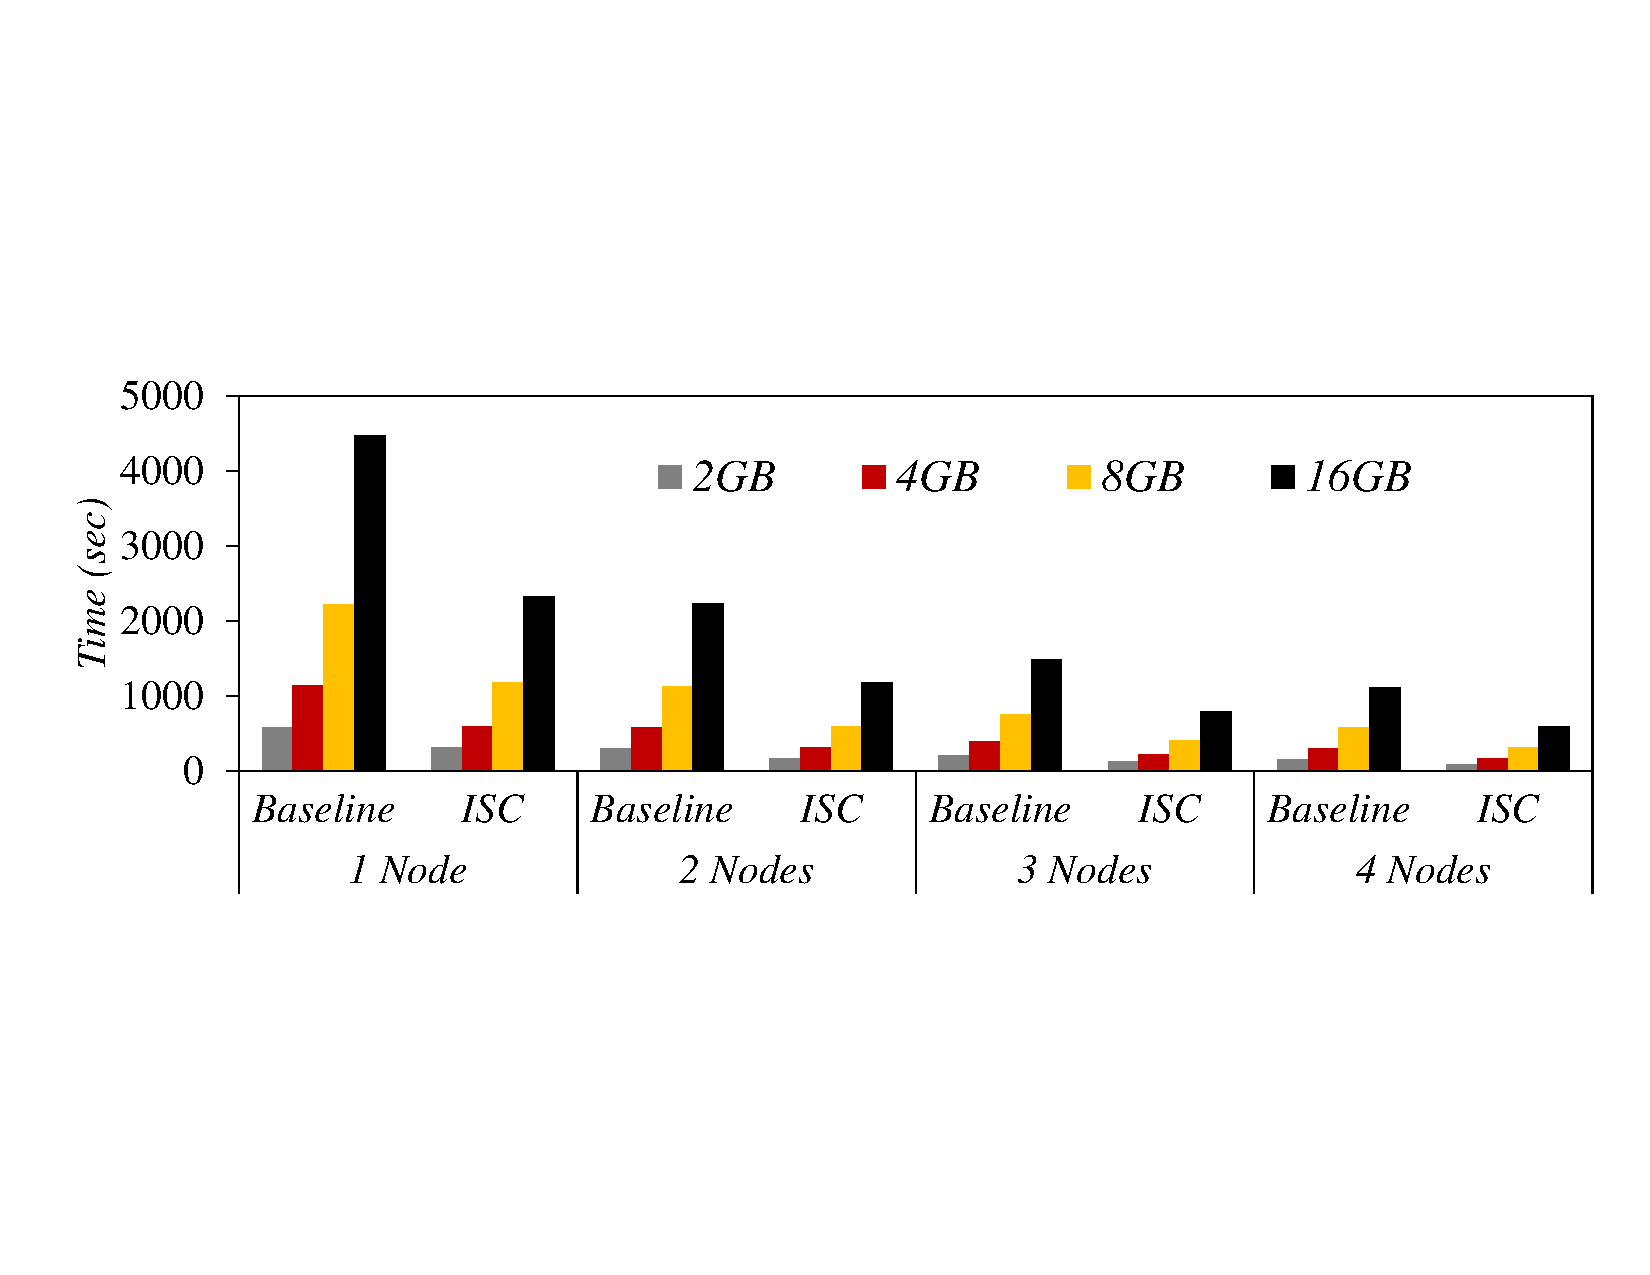
\includegraphics[width=1.25\columnwidth]{figures/Hadoop_total_execution_time_clusters.pdf}&
  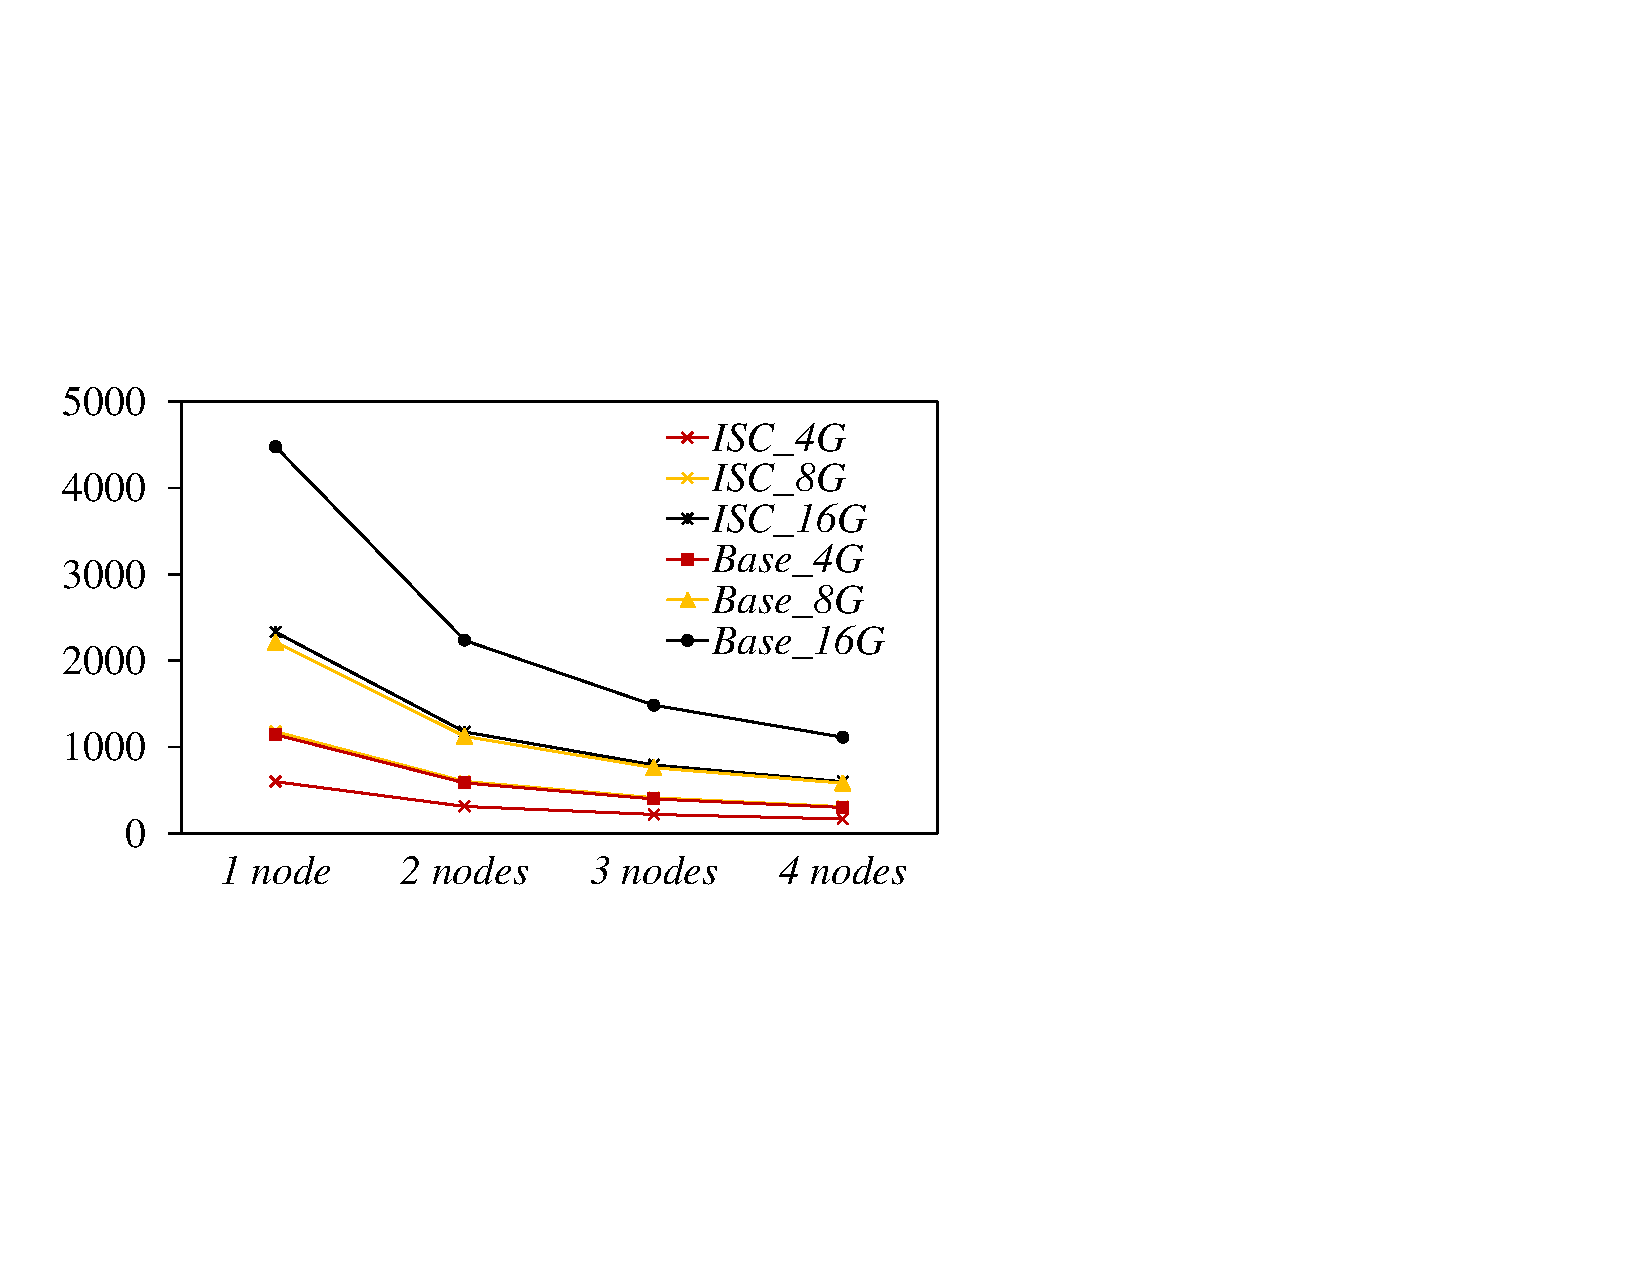
\includegraphics[width=0.75\columnwidth]{figures/Hadoop_total_execution_time_clusters_line.pdf}\\
  (a) Total Elapsed Time & (b) Total Elapsed Time 
\end{tabular}
  \caption{Total elapsed time on Hadoop clusters with a various number of datanode. A node here means datanode.}
  \label{fig:total_time_on_clusters}
\end{figure*}




\begin{figure*}[t]
  \centering
  \renewcommand{\tabcolsep}{2mm}
  \begin{tabular}{ccc}
 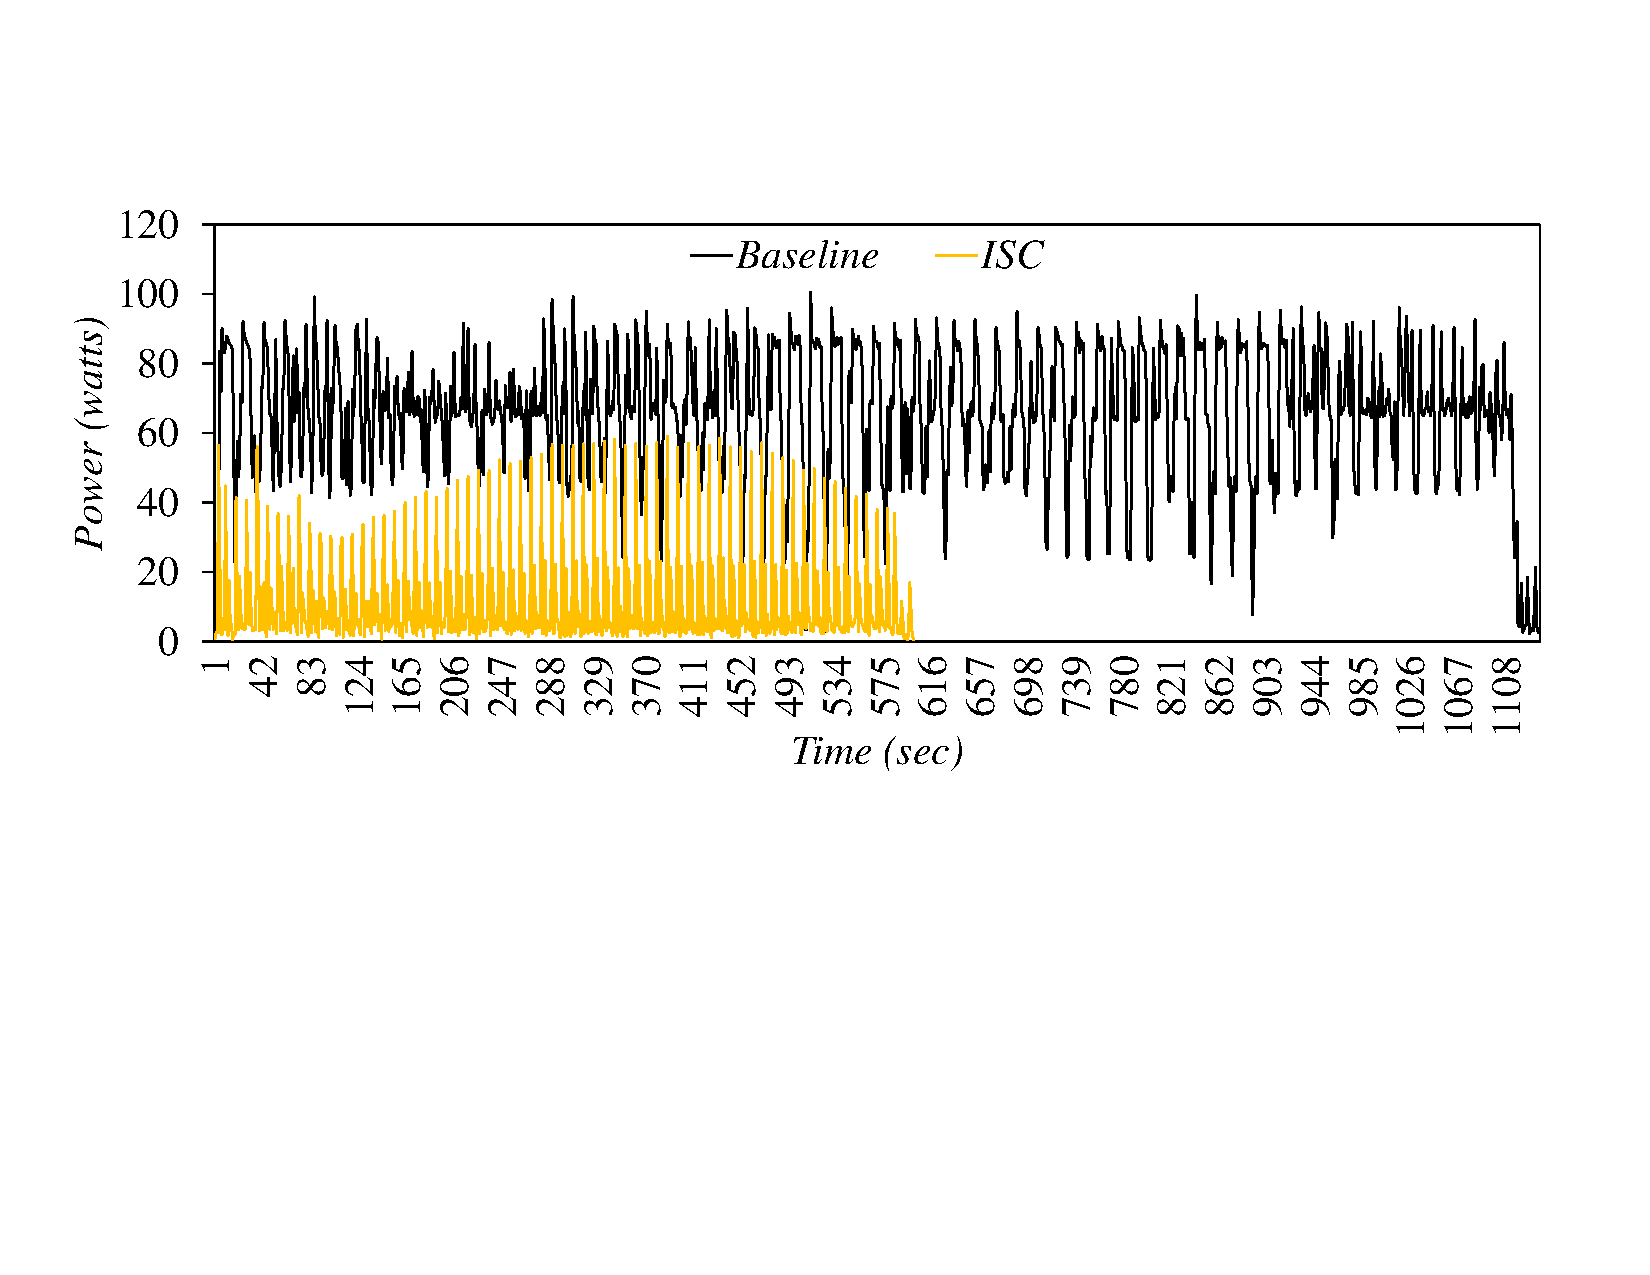
\includegraphics[width=1.25\columnwidth]{figures/Hadoop_power_clusters.pdf}&
  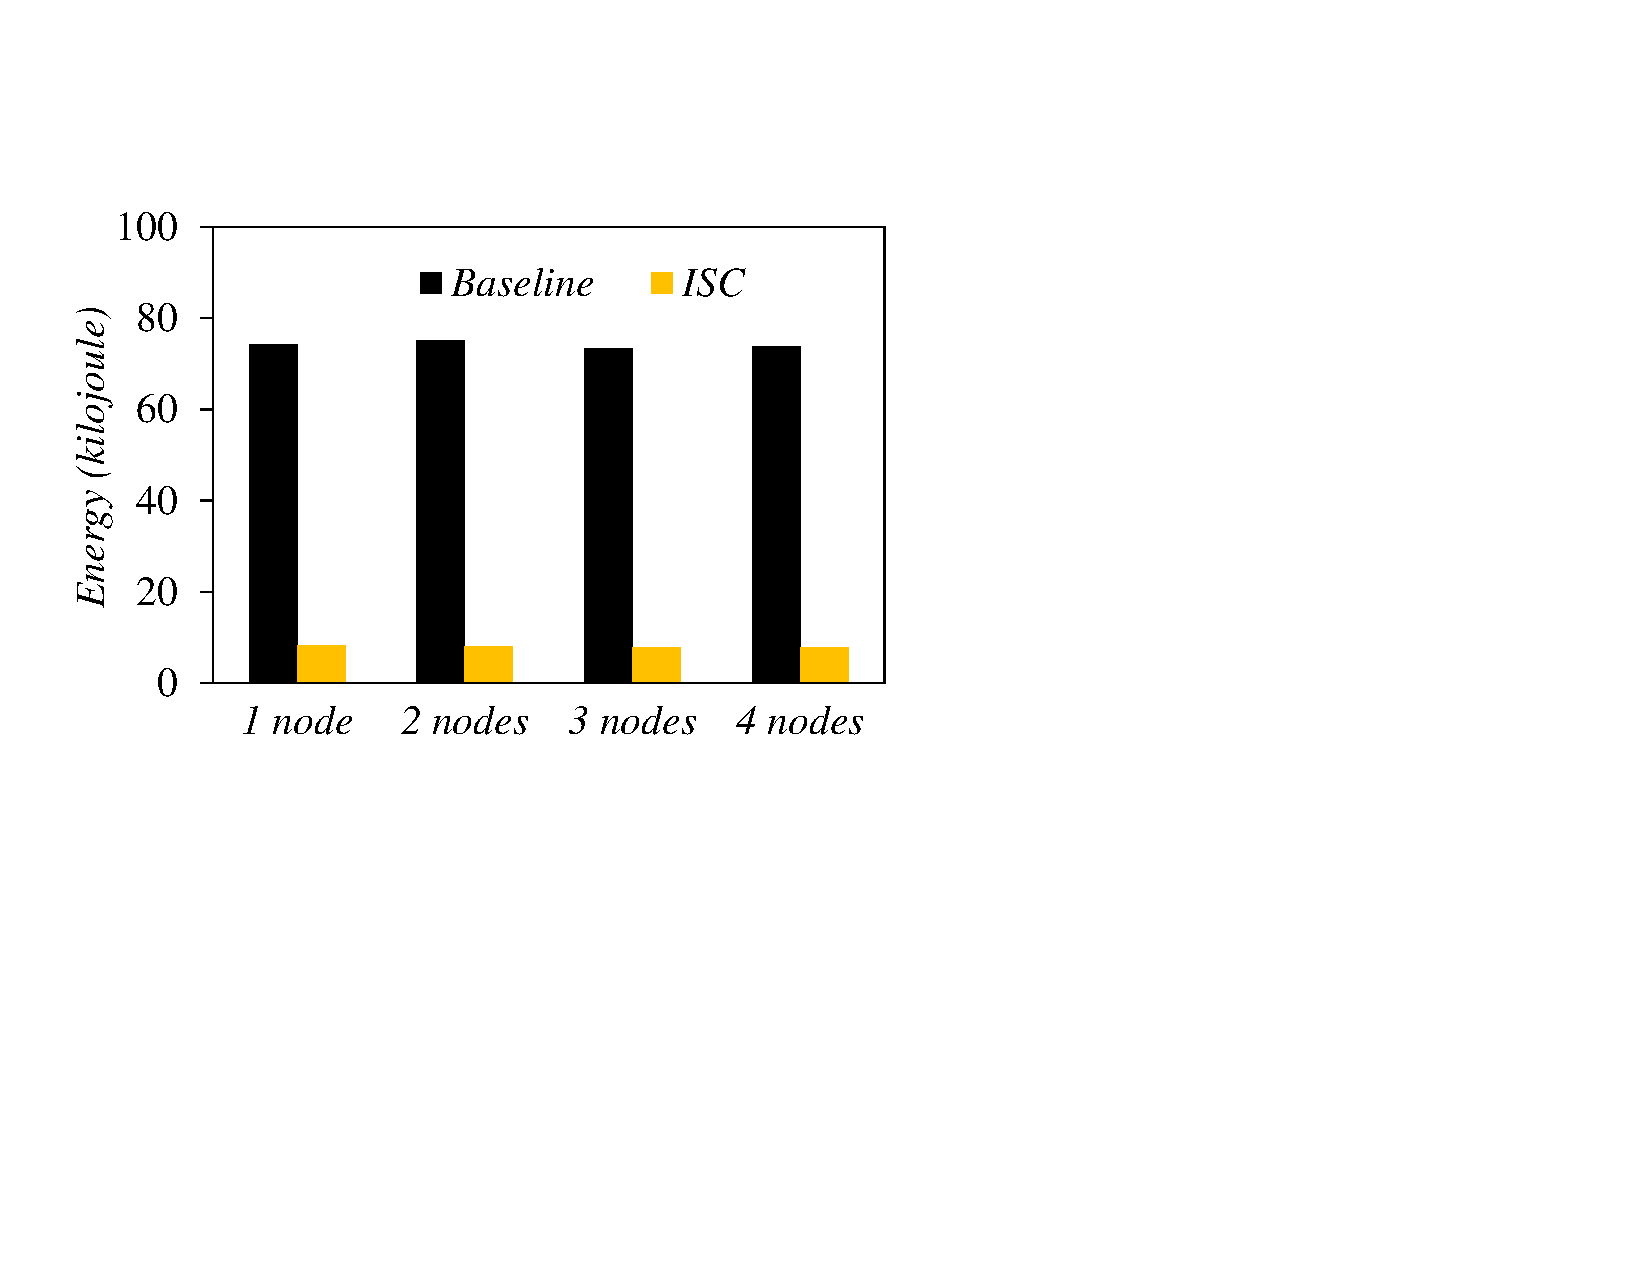
\includegraphics[width=0.75\columnwidth]{figures/Hadoop_energy_clusters.pdf}\\
  (a) Power Consumption Over Time (4 datanodes) & (b) Total Energy Consumption 
\end{tabular}
  \caption{Power and energy consumption on Hadoop clusters with 16GB data}
  \label{fig:total_energy_on_clusters}
\end{figure*}






\textbf{Host Read I/O:} Unlike a conventional CPU-centric system loading all data to the host for computation, an ISC system does not need to move data from a device to the host. This can significantly reduce Host I/O between them. Both Figure~\ref{fig:host_resource_usage} (b) and Figure~\ref{fig:avg_host_resource_usage} (b) support this claim. A typical Hadoop system generates lots of read I/Os to load all data from devices to the host, while our ISC Hadoop system very rarely generates read I/Os (almost 2 orders of magnitude less). Especially for the period of each Map task computation, the typical Hadoop system keeps reading data from the devices. This is also verified by our SATA/SAS bus analyzer (Figure~\ref{fig:ISC_Hadoop_demo}). We capture both read and write I/Os, but write I/Os are almost ignorable (less than 1\%) for this application. Thus, we exhibit only read I/Os in the plots. In addition, we also verified that when we add up all amounts of read I/Os, it is almost equivalent to the input data size of 1GB.






\textbf{Host DRAM Usage:} Host DRAM is another important factor to promote ISC systems. Typically, all data loaded from devices are first stored in host DRAM for computation, which results in a more memory consumption. To measure this host memory consumption, we do not run any other applications after reboot and flush all data/page caches. Thus, both starting points of the plot are almost the same. After running the Hadoop application, the baseline system keeps consuming DRAM until all Map tasks completes. On the other hand, our ISC Hadoop system consumes even less DRAM (3$\times$ less). This has a critical impact on energy consumption since it has been widely known that DRAM takes 25\% -- 40\% of a system power consumption~\cite{DRAM_Power:ISCA:2010,NewServerArch:ISCA:2008,PowerNap:ASPLOS:2009,DisaggregatedMem:ISCA:2009}.







\subsubsection{Hadoop Clusters}\label{subsubsec:Exp_result_clusters}
We set up clusters of 5 nodes (1 namenode and 4 datanodes) to verify whether or not all implications from a single node can be applied to real Hadoop clusters. Each datanode is equipped with a ISC device and connects to each others via 1Gb Ethernet switch. 
We run the same Hadoop application and data varying 1GB to 16GB (we eliminate results with 1GB in the plots). 

Figure~\ref{fig:total_time_on_clusters} (a) shows the total elapsed time on the clusters. The results are very similar to those on a single node: our ISC Hadoop system is 2$\times$ faster than baseline Hadoop system, which implies that ISC Hadoop clusters of a half size can achieve a similar performance to the baseline Hadoop clusters, or that ISC Hadoop clusters of the same size as the baseline Hadoop clusters can process two times amount of data for the same period of time. Figure~\ref{fig:total_time_on_clusters} (b) illustrates well this claim. For instance, the plot of the ISC Hadoop system with 16GB data (ISC\_16G) is almost overlapped with the plot of the baseline Hadoop system with 8GB data (Base\_8G).
We do not display the total Mapper elapsed time since the results are not so much different from the Figure~\ref{fig:total_time_on_clusters}. This is already verified in the Figure~\ref{fig:execution_time_with_single_namenode_on_single_node}.
 
As we analyzed in subsection~\ref{subsubsec:Exp_result_singlenode}, the total energy consumption of each size of clusters is almost identical (about 9.3$\times$ lower) since bigger clusters complete the same task with a shorter time (Figure~\ref{fig:total_energy_on_clusters} (b)). Note: like a sinle node experiment, we also eliminate an idle power. Figure~\ref{fig:total_energy_on_clusters} (a) plots a power consumption over time in the clusters of 4 datanodes (plus 1 namenode) with 16GB data. This shows that the ISC Hadoop system consumes about 4.6$\times$ lower power than the baseline system, which induces over 9$\times$ lower energy consumption considering 2$\times$ faster execution time.









%\begin{table}[tbp]
%\centering\small
%\begin{tabular}{l|l}\hline\hline
%\textbf{Parameters}  &   \textbf{Ranges}   \\\hline
%Number of lists & \textbf{2}, 3, 4, 5, 6, 7, 8\\\hline
%List size skewness factor  & 10000, 1000, \textbf{100}, 10, 1\\\hline
%Intersection ratio  &   0.1\%, \textbf{1\%}, 10\%, 100\%\\\hline
%List size & 1 MB, \textbf{10 MB}, 50 MB, 100 MB\\\hline\hline
%\end{tabular}
%\caption{Parameter setup}\label{tab:synData}
%\end{table}



%\begin{table}[tbp]\small
%\centering
%\begin{tabular}{l|l|l|l|l|l}\hline\hline
%$f$ & $n_1$ & $n_2$ & $n_p$ & estimated ANMP & real ANMP \\\hline
%$1$ & $327680$ & $327680$ & $2564$ & $\frac{n_1+n_2}{n_p}=256$ & $383$ \\\hline
%$10$ & $32768$ & $327680$ & $1408$ & $\frac{n_1\cdot\log n_2}{n_p}=427$ & $640$ \\\hline
%$100$ & $3277$ & $327680$ & $1284$ & $\frac{n_1\cdot\log n_2}{n_p}=47$ & $68$ \\\hline
%$1000$ & $328$ & $327680$ & $1280$ & $\frac{n_1\cdot\log n_2}{n_p}=5$ & $6$ \\\hline\hline
%\end{tabular}
%\caption{The average number of memory accesses per page (ANMP) in Figure~\ref{fig:varyListSkewIntersection}, where $f$ means the skewness factor, $n_1$ and $n_2$ indicate the number of entries in list $A$ and $B$, $n_p$ is the total number of pages. Note that each page is 8 KB and each entry takes 32 bytes. Thus, each page can contain 256 entries.}\label{tab:varyListSkewIntersection}
%\end{table}





%  \begin{figure}[tbp]
%  \centering
%    \begin{tabular}{ccc}
% 
\includegraphics[width=0.52\columnwidth]{figures/banner2.pdf}
%\end{tabular}
%\vspace{-0.1cm}
%\renewcommand{\tabcolsep}{0.1mm}
%  \begin{tabular}{ccc}
% 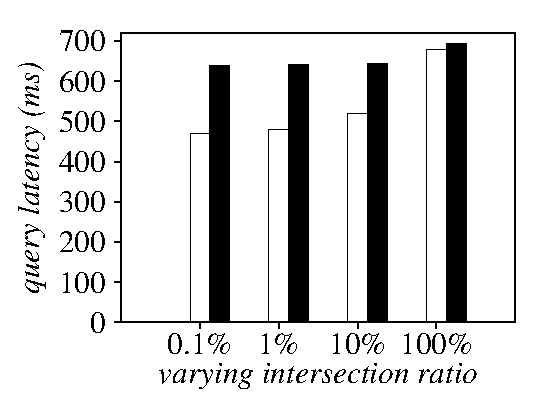
\includegraphics[width=0.5\columnwidth]{figures/Intersection-time-VaryInterRatio-equal2.eps}&
%  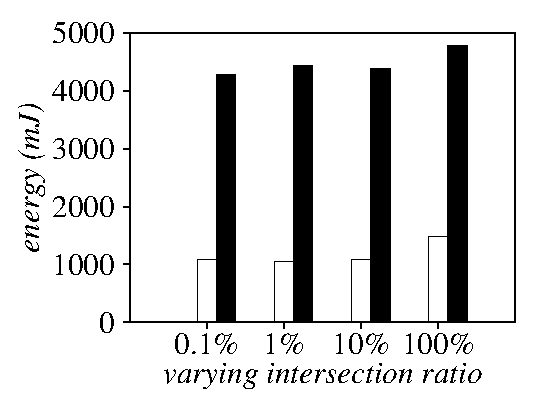
\includegraphics[width=0.5\columnwidth]{figures/Intersection-energy-VaryInterRatio-equal2.eps}\\
%  (a) query latency & (b) energy\\
%\end{tabular}
%  \caption{Varying intersection ratio on equal-sized lists (for intersection)}
%  \label{fig:varyInterRatioIntersection2}
% \end{figure}



%\subsubsection{Discussion: Call for Algorithmic Optimizations}\label{sec:rankUnionOpt}
%Because of too many memory accesses, it is not cost-effective to offload ranked union to Smart SSD.
%To resolve this limitation, on the one hand, we fundamentally need to improve the innate memory access speed of Smart SSDs through the hardware upgrade. On the other hand, more efficient algorithms could be designed to reduce memory access. Our current implementation (following Lucene) solves the ranking problem only if all the union results are available, then scores every qualified document. However, both union and ranking could be algorithmically combined for early termination~\cite{Broder2003EQE,Fagin2001}. This means we do not need to scan all the union results. We will explore the early pruning techniques in the future work. \textcolor{red}{Can delete if no space}

%Because of too many memory accesses, it is not cost-effective to offload ranked union to Smart SSD. To resolve this limitation, on the one hand, we fundamentally need to improve the innate memory access speed of Smart SSD through its hardware update. On the other hand, more efficient algorithms could be designed to reduce memory access. Our current implementation (following Lucene) solves the ranking problem when all the union results are available, then scores every qualified document. However, union and ranking could be algorithmically combined for early termination~\cite{Broder2003EQE,Fagin2001}. Meaning that, we do not need to scan all the union results. We will explore the early pruning techniques in the future work.


%More importantly, one needs to be careful about the \emph{hidden constant} of algorithms, not only big O notation. E.g., the sort-merge based union algorithm is in linear cost, however, the hidden constant factor slows down the performance significantly.



%\textbf{Algorithmically combined (may be a possible)\cite{topk}.}

%\textbf{A special case of ranked union on \emph{two} lists.} If the number of lists is 2, a better algorithm for Smart SSD can be as follows. (1) Find the intersection results $R$ between $k$ lists $L_1, L_2, \cdots, L_k$. It takes, usually, less than 1 scan of all lists; (2) Scan Scan $R$, and $L_1, L_2, \cdots, L_k$ to find the top ranked results. It takes 1 scan. Thus, in total, around 2 full scans on all the $k$ lists. In this case, Samrt SSD wins.
